 
\begin{anexosenv}
\partanexos
\chapter{Prot\'otipo}
\pagestyle{simple}
\label{cap:manual}

\section{Instalação}

\subsection{Pré-requisitos do Projeto}

Programas necessários para realizar a utilização do \textit{software}:

\begin{itemize}
    \item \textbf{Apache Server}.
    \item \textbf{PHP} \textit{7.0 ou superior}.
    \item \textbf{MariaDB} \textit{10 ou superior}.
    \item \textbf{GIT}.
\end{itemize}

Após verificar a existência dos programas citados e suas respectivas versões, pode ser iniciado o processo de instalação.

Para realizar a instalação deve-se entrar no diretório indicado pelo servidor \textbf{Apache} no seu sistema operacional através terminal (ou \textit{console}), e após isso executar os comandos de acordo com o tutorial contido no repositório do protótipo  \url{http://github.com/FilipeRodrigues3003/TCC/agendador}. Com isso você irá copiar os arquivos do protótipo para o diretório do seu servidor local.


\section{Utilização}

Após a instalação pode-se acessar o software a partir de \url{//localhost/agendador} para acessar o protótipo em caso de instalação seu próprio computador, ou através de \url{http://ipdoseuservidor/agendador} caso tenha feito a instalação em um servidor remoto.

Ao acessar pela primeira vez será exibida a página de \textit{\textbf{Login}} conforme figura \ref{tela-login} abaixo, caso o usuário ainda não possua um \textit{login}, este deverá clicar sobre o botão \textbf{Cadastre-se}.

%% Tela Login
\begin{figure}[H]
     \centering
     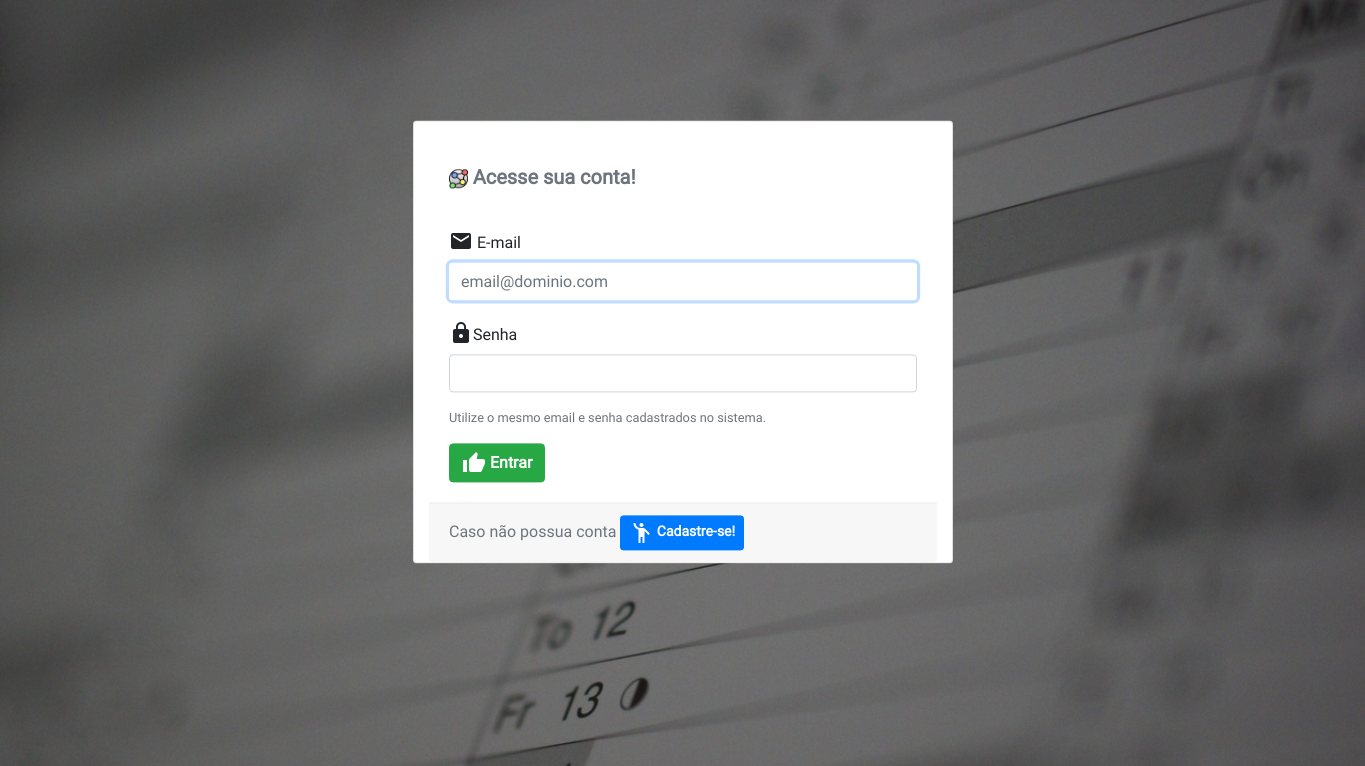
\includegraphics[width=0.8\textwidth]{TCC/imagens/sistema/01.png}
     \caption{Tela de Login}
     \label{tela-login}
\end{figure}

\subsection{Cadastro de Usuários}

Para que seja possível utilizar o sistema, é necessário que o usuário possua um \textit{login} no mesmo, e para isso o usuário deverá realizar um pequeno cadastro na página apresentada na figura \ref{tela-cadastro-usuario}. 

O usuário deverá informar obrigatoriamente: seu nome completo, endereço de \textit{e-mail} válido e uma senha.

%% Tela Cadastro de Usuário
\begin{figure}[H]
     \centering
     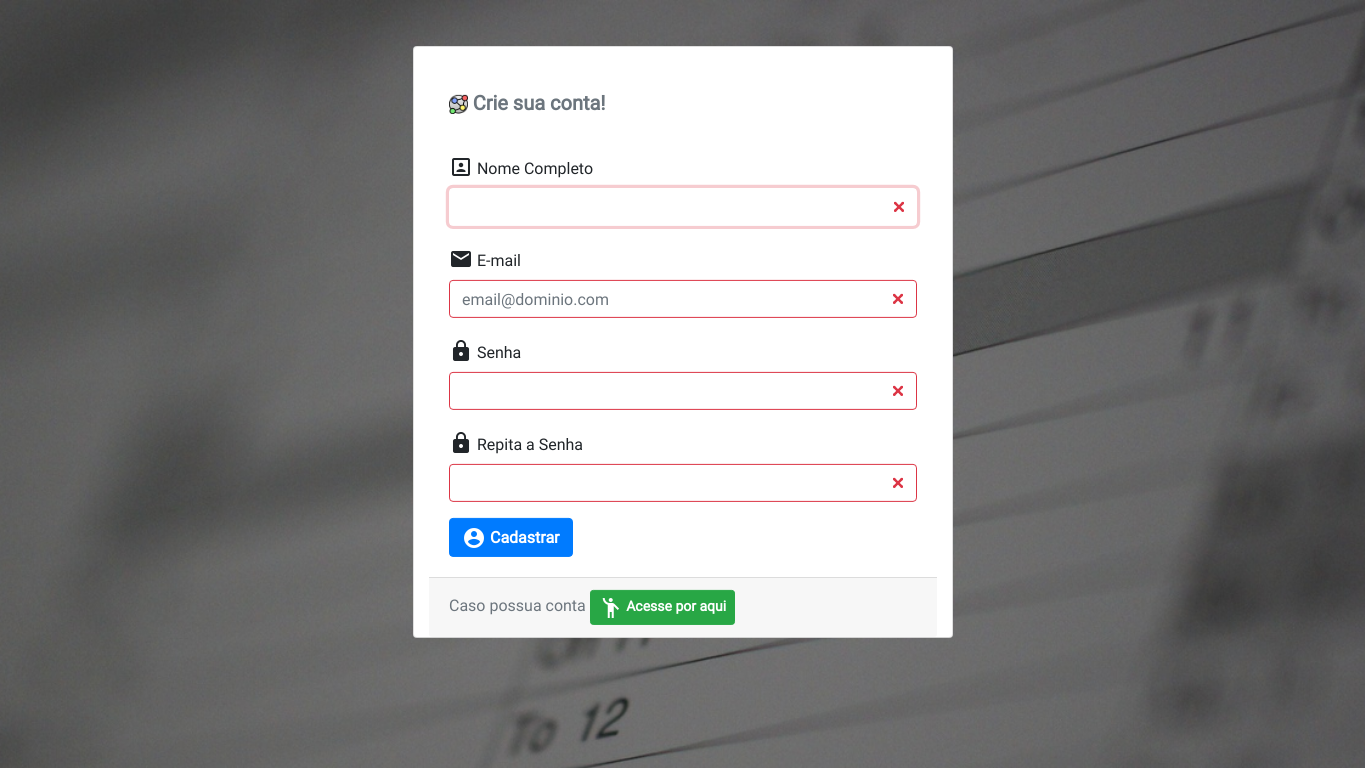
\includegraphics[width=0.8\textwidth]{TCC/imagens/sistema/02.png}
     \caption{Tela de Cadastro de Usuário}
     \label{tela-cadastro-usuario}
\end{figure}

A partir do momento em que o usuário realizar seu cadastro, será possível efetuar \textit{login} no sistema. Para isso o usuário deverá submeter seu \textit{e-mail} e senha (conforme informado no cadastro).


\subsection{Dashboard}

Após efetuar o \textit{login}, o usuário estará na tela de \textbf{Dashboard} do sistema, na qual visualizará seus \textbf{espaços de trabalho}, o \textbf{menu de navegação principal}, no topo da página, além da opção de \textbf{criar novos espaços de trabalho}.

%% Tela de Dashboard
\begin{figure}[H]
     \centering
     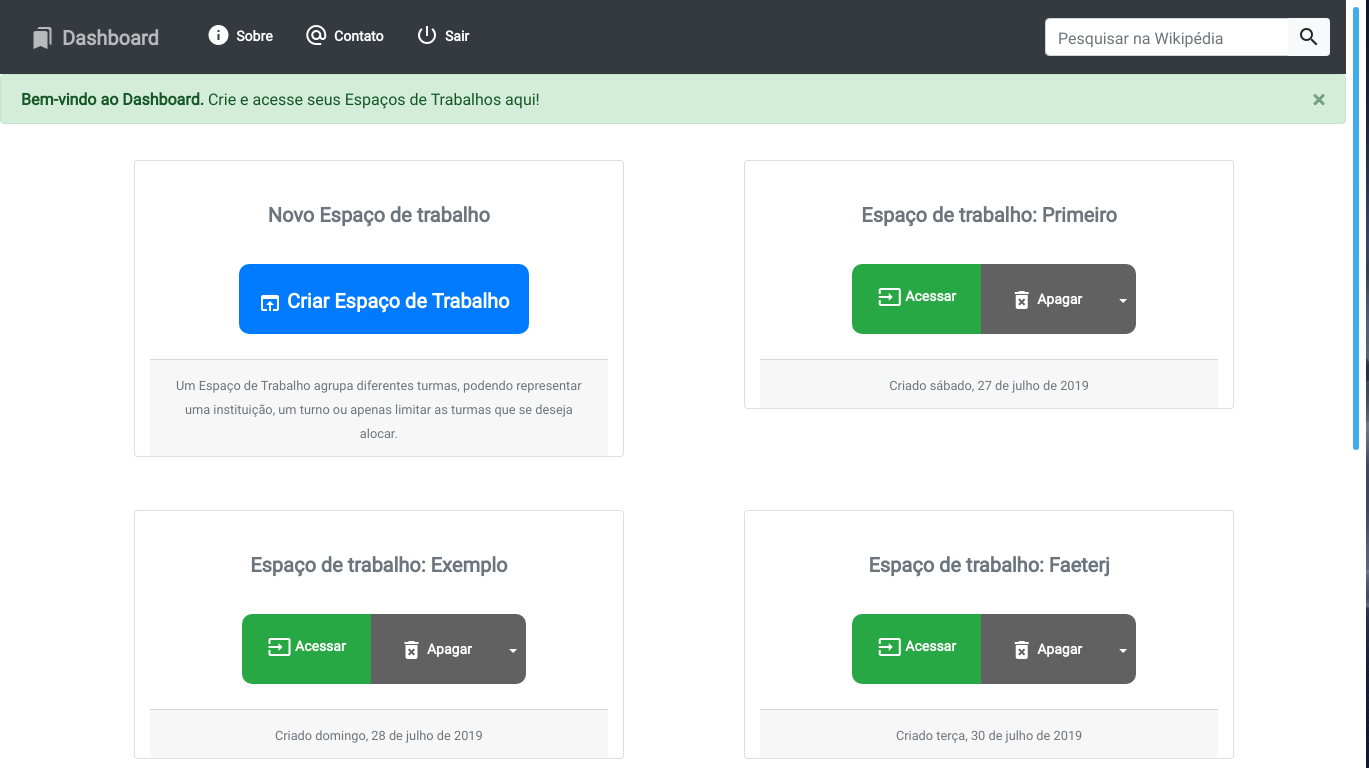
\includegraphics[width=0.8\textwidth]{TCC/imagens/sistema/03.png}
     \caption{Tela de Dashboard}
     \label{tela-dashboard}
\end{figure}

Um \textbf{espaço de trabalho} aqui é análogo a uma instituição, turno ou qualquer outra forma pela qual o usuário deseja separar as turmas que deverão ter as grades de prova geradas.

Para se \textbf{criar um novo espaço de trabalho} deve-se clicar no botão azul escrito "Criar Espaço de Trabalho"\ no \textit{\textbf{Dashboard}}, e informar o nome que o espaço de trabalho deverá ter, como mostrado na figura \ref{tela-new-workspace}.
%% Tela Login
\begin{figure}[H]
     \centering
     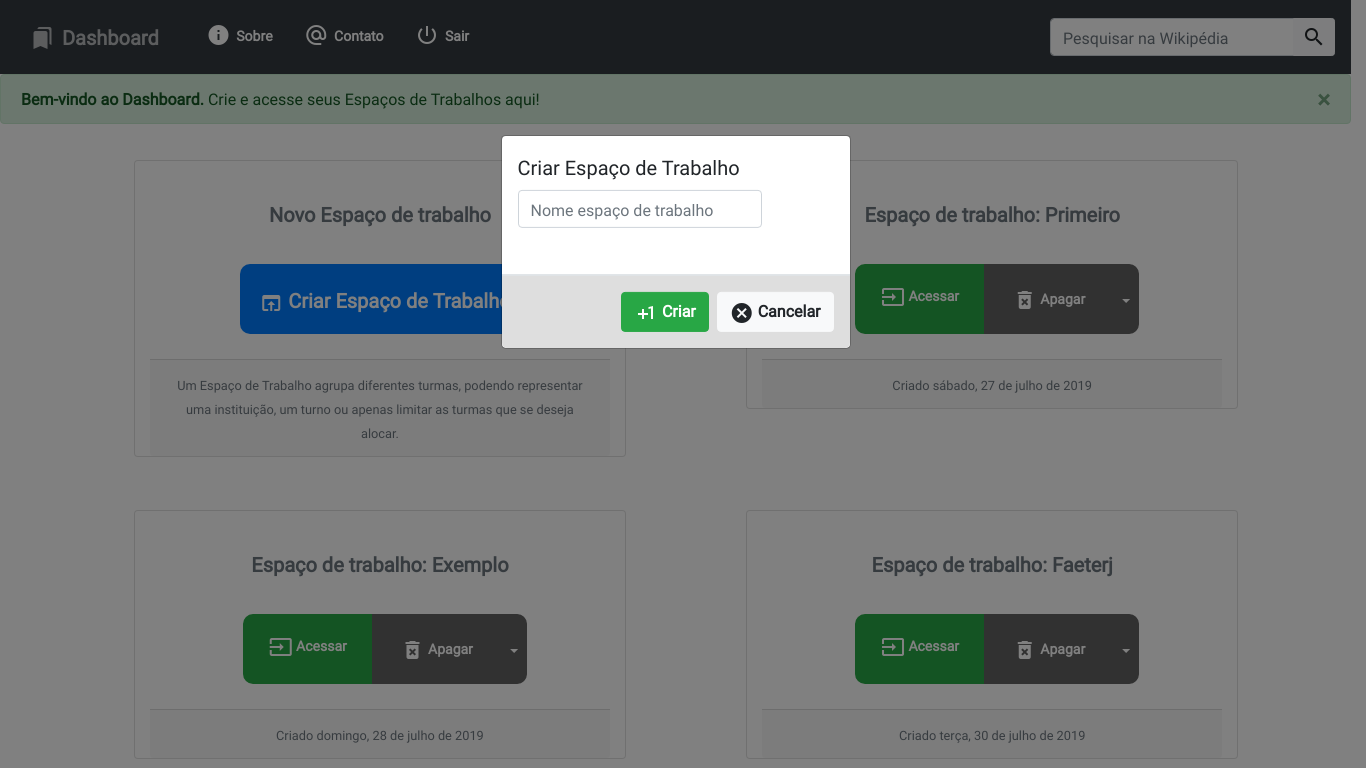
\includegraphics[width=0.8\textwidth]{TCC/imagens/sistema/03b.png}
     \caption{Tela de Criação de Novo Espaço de Trabalho}
     \label{tela-new-workspace}
\end{figure}

No canto direito do \textbf{menu de navegação principal} temos uma barra de pesquisa, que serve para auxiliar o usuário em caso de dúvidas com termos técnicos, fazendo consultas diretamente na enciclopédia online \url{Wikepédia.org} observado na figura \ref{tela-wiki}, possibilitando dessa forma esclarecer as dúvidas sem ser necessário deixar a tela do sistema como apresentado na figura \ref{tela-popup}.
%% Tela Login
\begin{figure}[H]
     \centering
     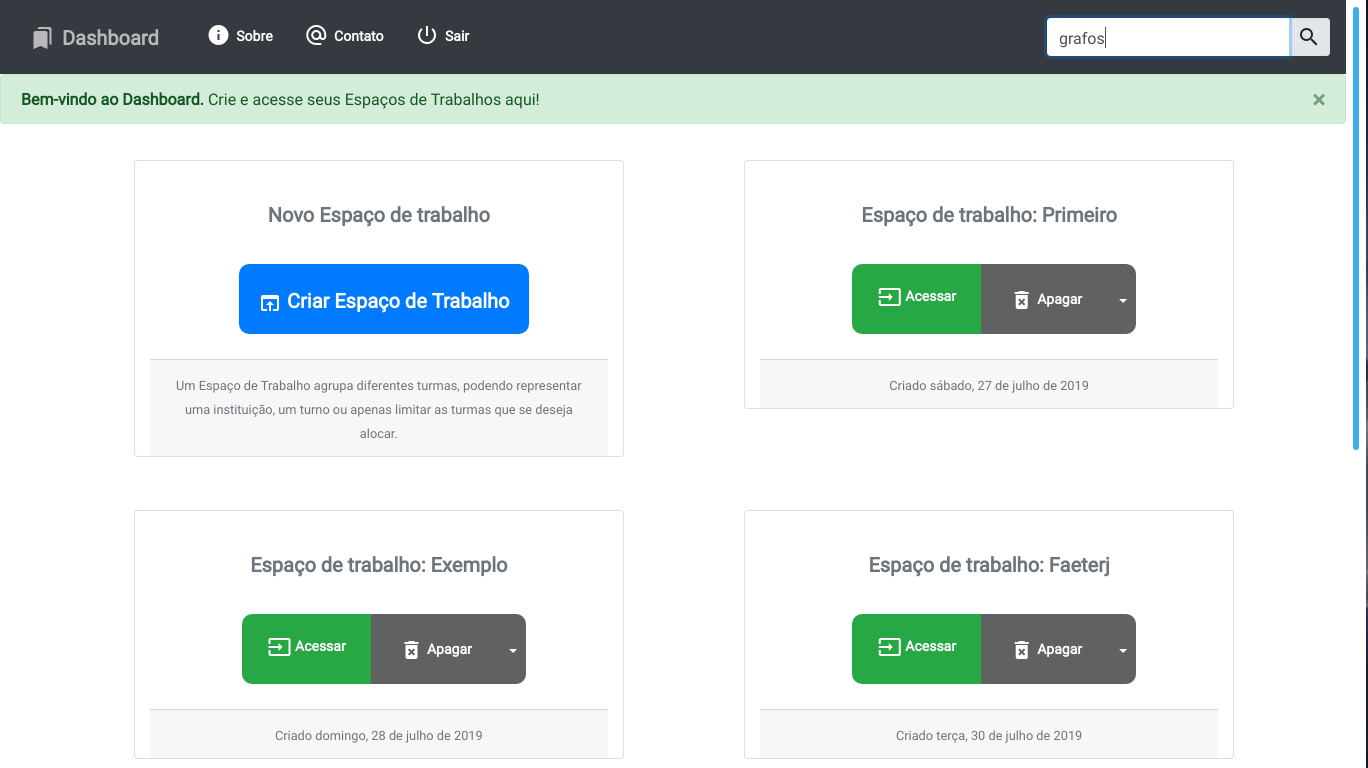
\includegraphics[width=0.8\textwidth]{TCC/imagens/sistema/03c.png}
     \caption{Tela de Campo de Busca na Wikipédia}
     \label{tela-wiki}
\end{figure}

%% Tela Login
\begin{figure}[H]
     \centering
     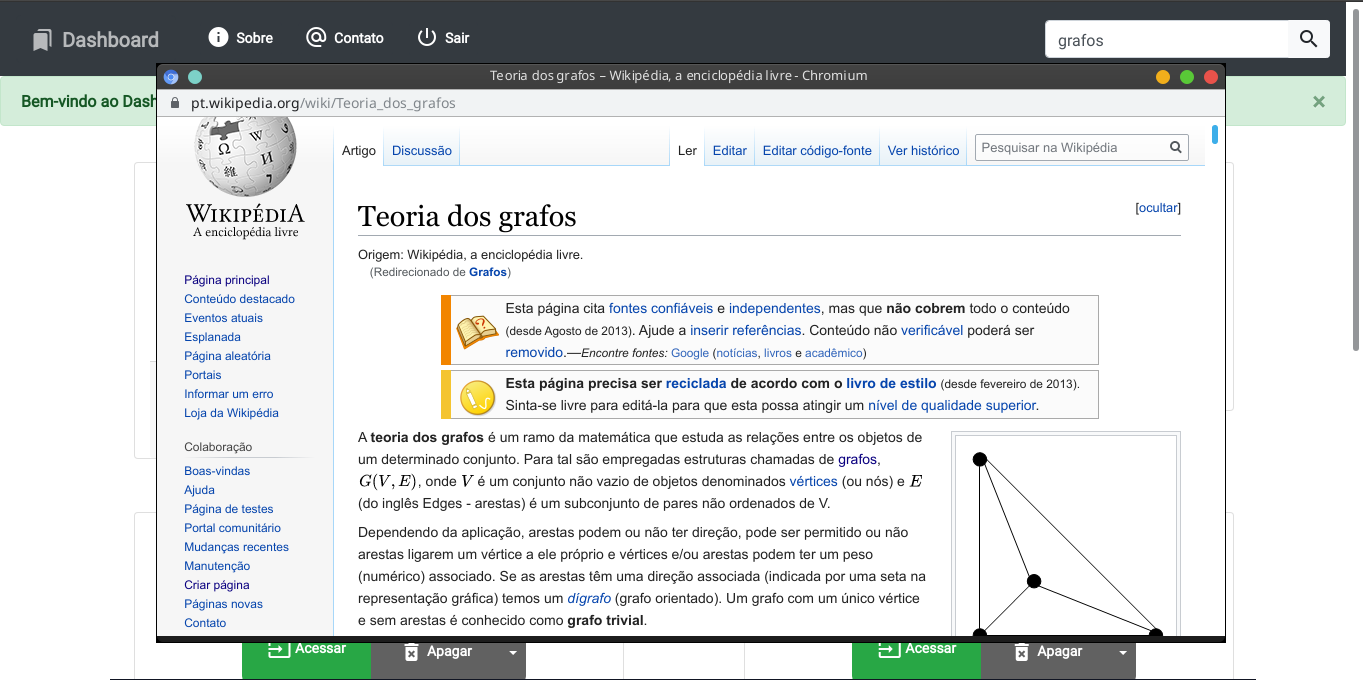
\includegraphics[width=0.8\textwidth]{TCC/imagens/sistema/03d.png}
     \caption{Tela de Campo de Busca na Wikipédia Pop-up}
     \label{tela-popup}
\end{figure}

Ainda no \textbf{menu de navegação principal}, da esquerda para direita observamos as seguintes opções:

Em \textbf{Sobre} que apresentará informações sobre o sistema, como o autor, os objetivos do projeto e como foi realizado o desenvolvimento do protótipo, assim como vemos na figura \ref{tela-sobre}
%% Tela Login
\begin{figure}[H]
     \centering
     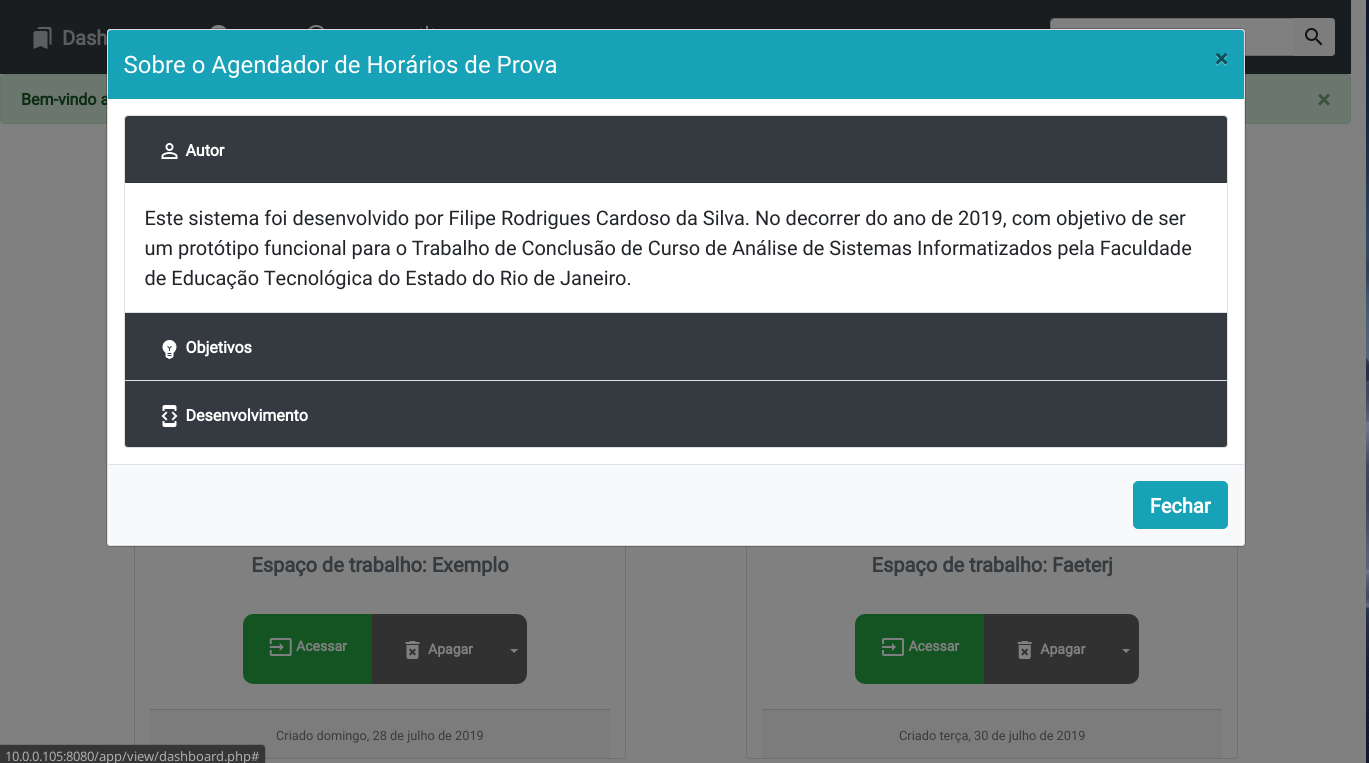
\includegraphics[width=0.8\textwidth]{TCC/imagens/sistema/04.png}
     \caption{Tela Sobre o Sistema}
     \label{tela-sobre}
\end{figure}

Em sequencia temos a opção \textbf{Contato}, que permite o envio de um \textit{e-mail},  conforme visto na figura \ref{tela-contato}, enviando-o para o desenvolvedor do sistema, para informar de possíveis problemas ou possibilitar o contato por qualquer que seja o motivo.
%% Tela Login
\begin{figure}[H]
     \centering
     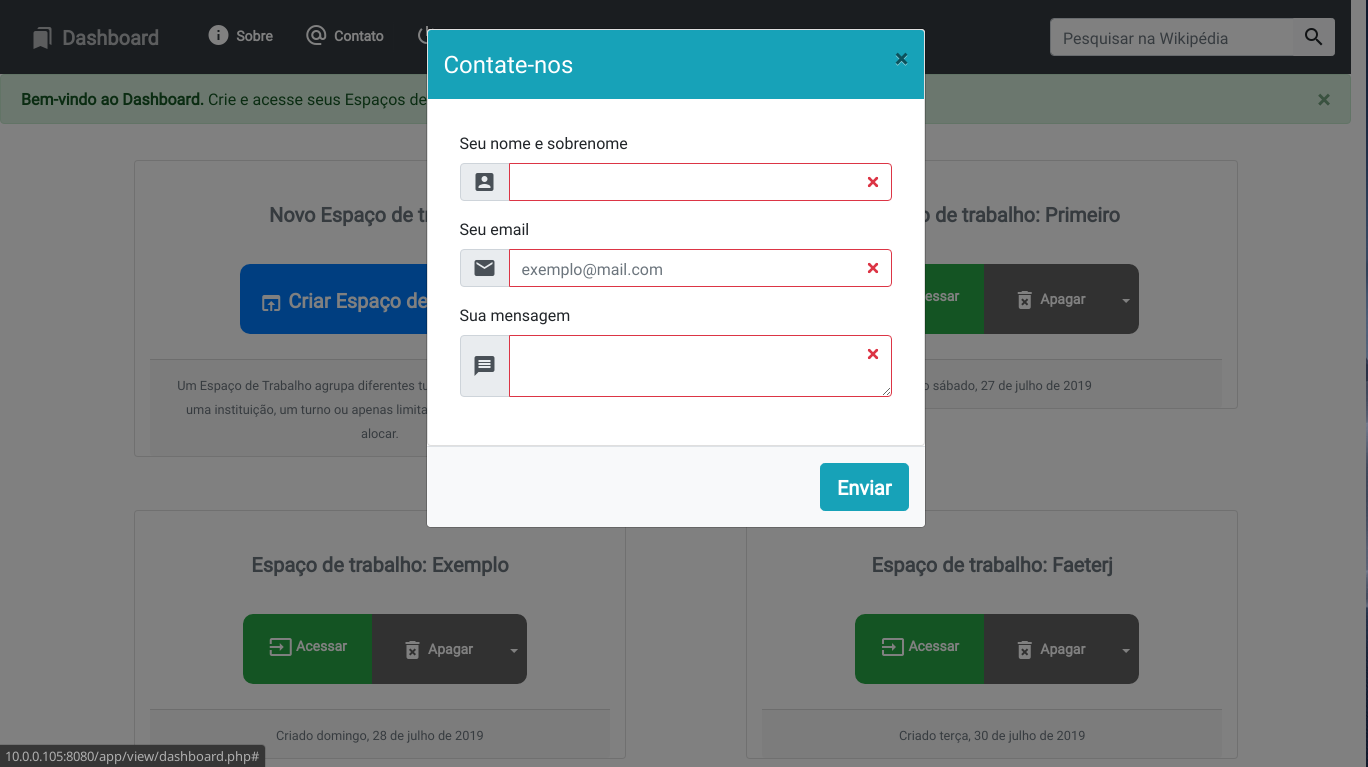
\includegraphics[width=0.8\textwidth]{TCC/imagens/sistema/05.png}
     \caption{Tela de Contato}
     \label{tela-contato}
\end{figure}

No \textbf{\textit{Dashboard}} temos ainda em cada espaço de trabalho as opções de acessar, apagar e um menu flutuante, como mostrada na figura \ref{tela-opcoes-rapidas}, com opções adicionais, facilitando o acesso à algumas funcionalidades do espaço de trabalho como importar e exportar as turmas presentes sem precisar acessar o espaço de trabalho.

%% Tela Login
\begin{figure}[H]
     \centering
     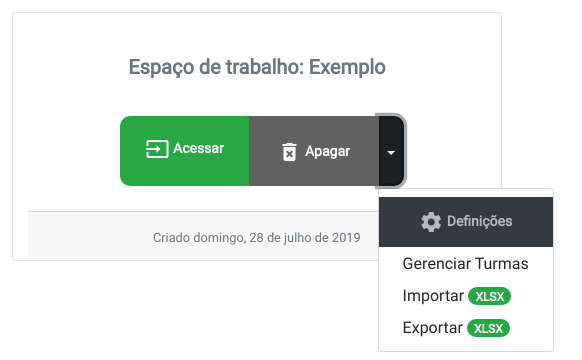
\includegraphics[width=0.8\textwidth]{TCC/imagens/sistema/06.png}
     \caption{Opções Rápidas do Espaço de Trabalho}
     \label{tela-opcoes-rapidas}
\end{figure}

\subsection{Definições do Espaço de Trabalho}

Ao acessar um espaço de trabalho, o usuário é redirecionado para a tela de \textbf{Definições do Espaço de Trabalho}, na qual é possível acessar as opções de configuração daquele espaço.

Dentre as suas opções (figura \ref{tela-definicoes}) temos a opção de criar uma tabela de horários, gerenciar as turmas pertencentes ao espaço de trabalho, adicionar turmas manualmente ou por arquivo (como visto na figura \ref{tela-definicoes-2}) ou exportar as turmas do espaço (figura \ref{tela-definicoes-3}), ainda temos a opção \textbf{Robô}, que demonstra uma explicação do que é o "Robô"\ usado no sistema (figura \ref{tela-robo}).

%% Home 1
\begin{figure}[H]
     \centering
     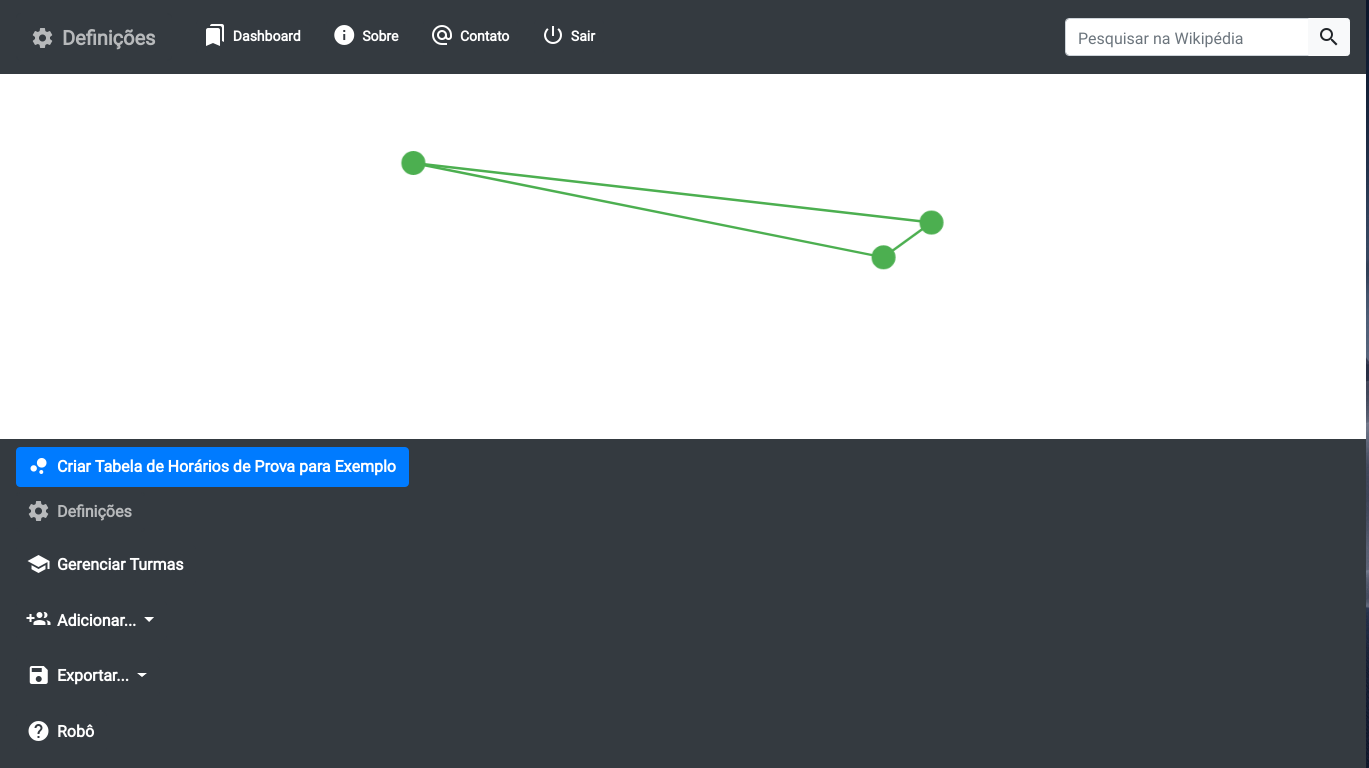
\includegraphics[width=0.8\textwidth]{TCC/imagens/sistema/07.png}
     \caption{Tela de Definições do Espaço de Trabalho}
     \label{tela-definicoes}
\end{figure}

%% Home 2
\begin{figure}[H]
     \centering
     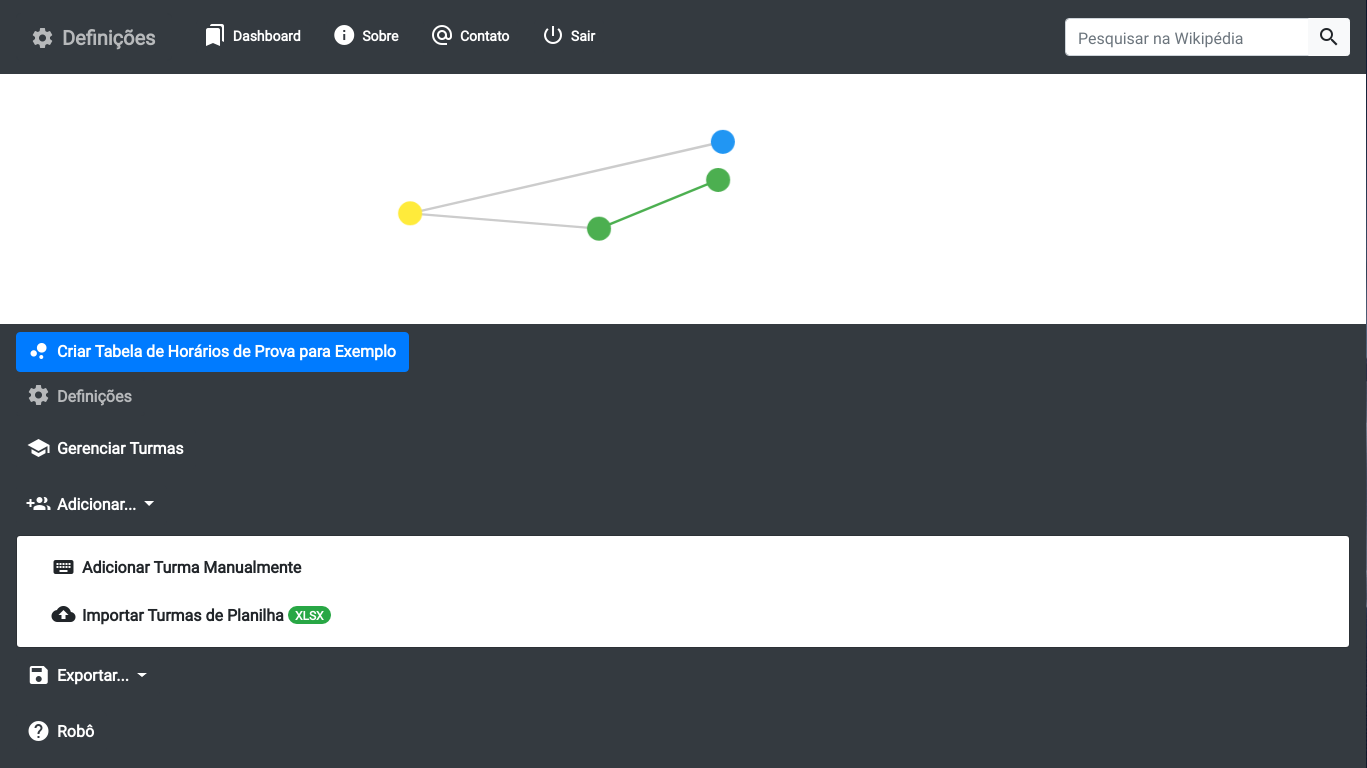
\includegraphics[width=0.8\textwidth]{TCC/imagens/sistema/07b.png}
     \caption{Tela de Definições do Espaço de Trabalho - Caixa de Seleção para Adicionar Dados}
     \label{tela-definicoes-2}
\end{figure}

%% Home 3
\begin{figure}[H]
     \centering
     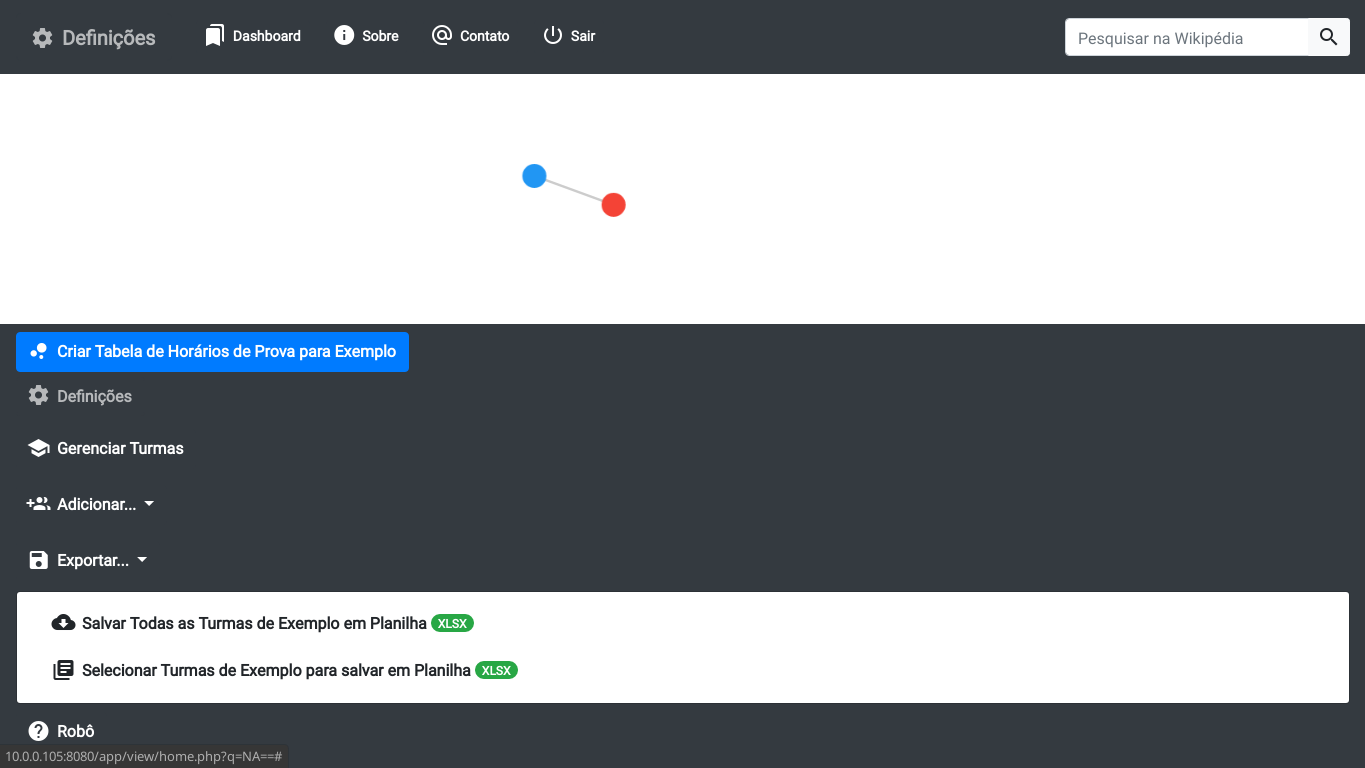
\includegraphics[width=0.8\textwidth]{TCC/imagens/sistema/07c.png}
     \caption{Tela de Definições do Espaço de Trabalho - Caixa de Seleção para Exportar Dados}
     \label{tela-definicoes-3}
\end{figure}

%% Home 4
\begin{figure}[H]
     \centering
     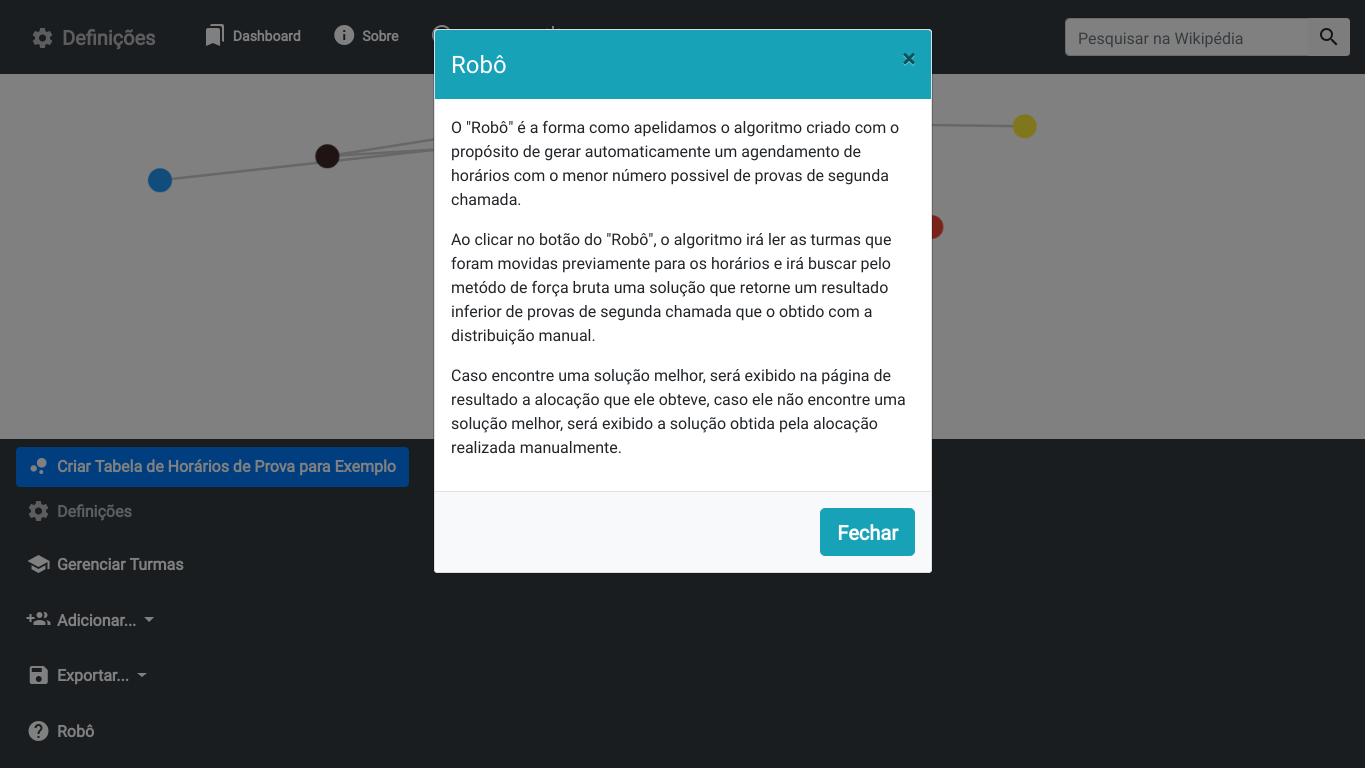
\includegraphics[width=0.8\textwidth]{TCC/imagens/sistema/07d.png}
     \caption{Tela de Explicação da Solução através do uso do Robô}
     \label{tela-robo}
\end{figure}

\subsection{Gerenciar Turmas}

Ao acessar a opção de \textbf{Gerenciar Turmas}, o usuário é direcionado para a página em que visualizará as turmas que estão presentes naquele espaço de trabalho (figura \ref{tela-gerenciador}). Nesta página o usuário poderá \textbf{adicionar uma turma}, e caso já tenha adicionado turmas, terá as opções de visualizar, editar e apagar as turmas e seus alunos.

Quando selecionada a opção de \textbf{visualizar turma}, o usuário tem acesso a uma listagem de alunos que pertencem aquela turma (figura \ref{tela-visu-1}), a opção de retornar a tela de gerenciamento de turmas, e a de edição da turma (figura \ref{tela-visu-2}).
%% Gerenciar turmas
\begin{figure}[H]
     \centering
     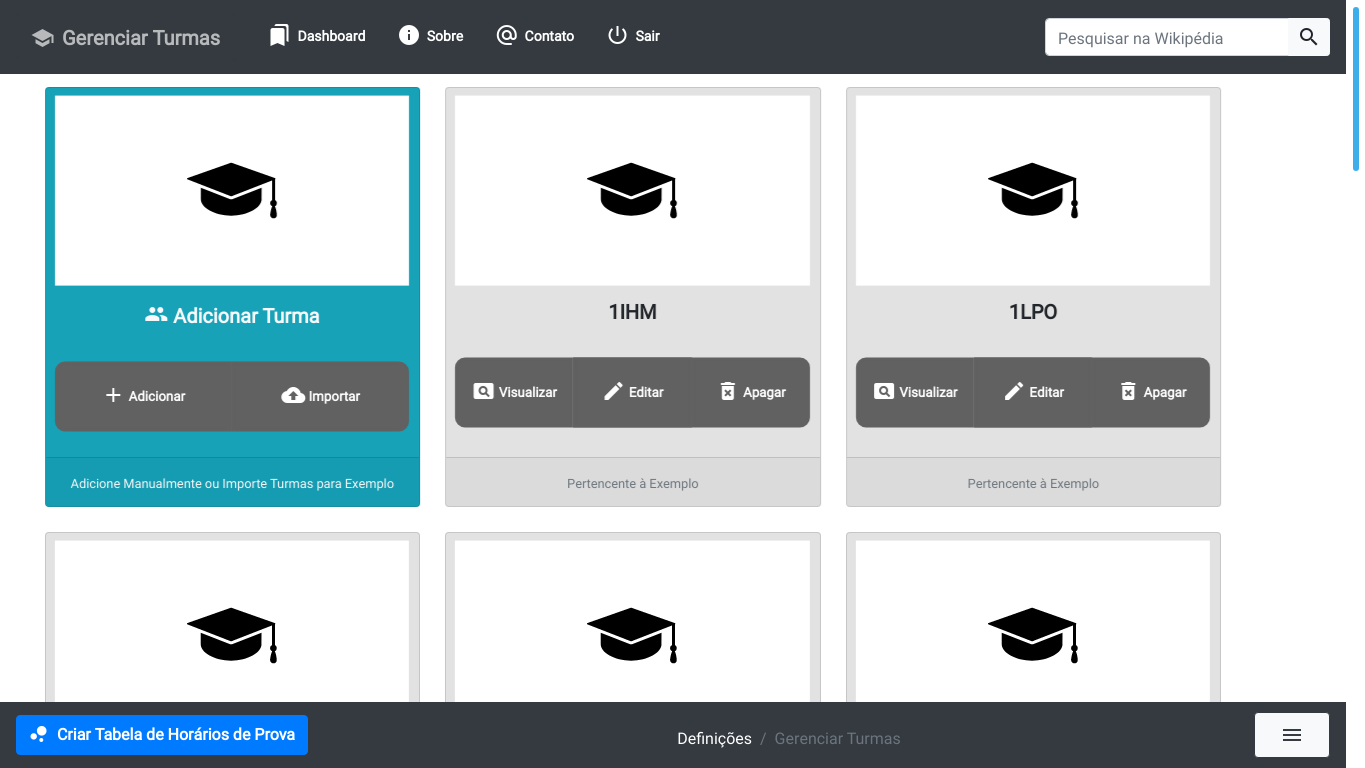
\includegraphics[width=0.8\textwidth]{TCC/imagens/sistema/08.png}
     \caption{Tela de Gerenciamento de Turmas}
     \label{tela-gerenciador}
\end{figure}

%% Visualizar alunos da turma 1
\begin{figure}[H]
     \centering
     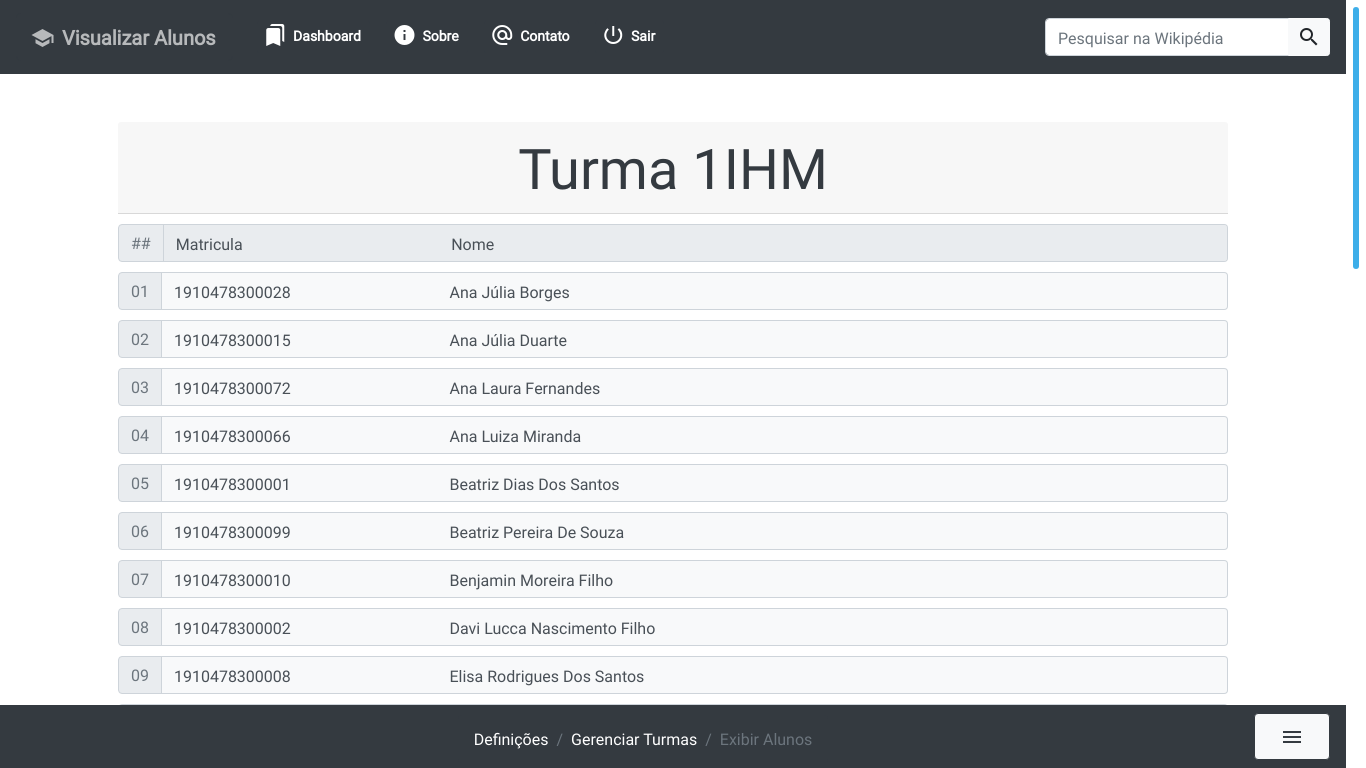
\includegraphics[width=0.8\textwidth]{TCC/imagens/sistema/09.png}
     \caption{Tela de Visualização da Turma}
     \label{tela-visu-1}
\end{figure}

%% Visualizar alunos da turma 2
\begin{figure}[H]
     \centering
     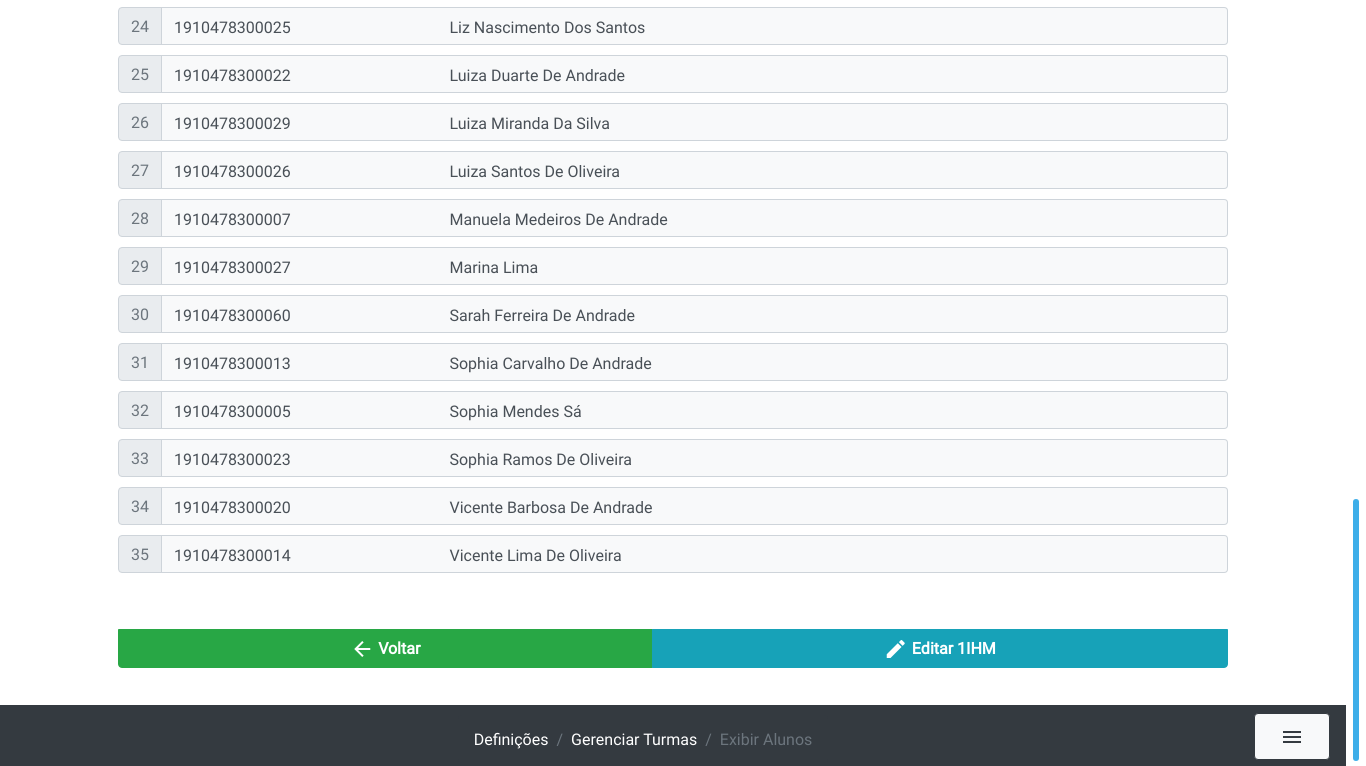
\includegraphics[width=0.8\textwidth]{TCC/imagens/sistema/09b.png}
     \caption{Tela de Visualização da Turma -- Cont.}
     \label{tela-visu-2}
\end{figure}

Para se \textbf{editar uma turma}, o usuário será direcionado para a página de edição (figura \ref{tela-edit-1}), onde poderá modificar a matrícula ou nome de um aluno em especifico, remove-lo da turma ou adicionar um novo aluno na turma (figura \ref{tela-edit-2}).


%% Editar alunos da turma 1
\begin{figure}[H]
     \centering
     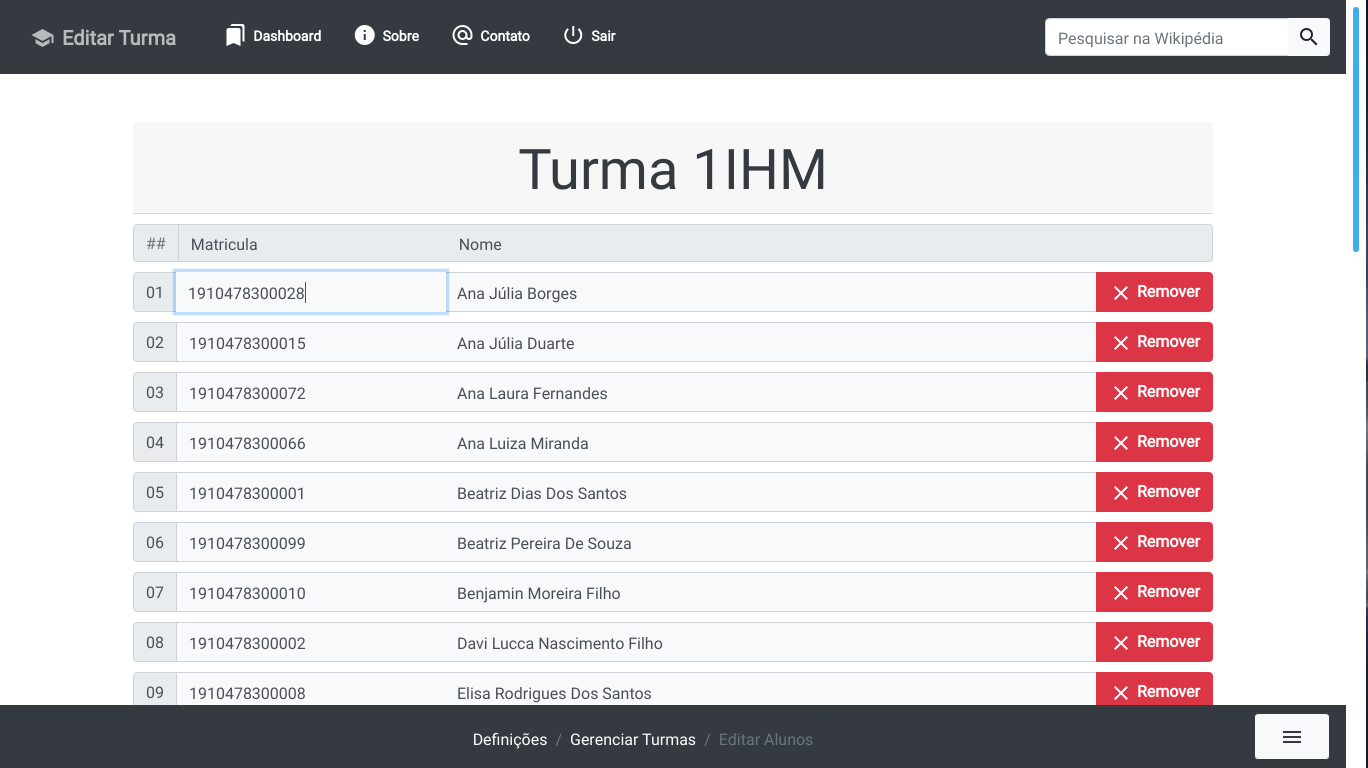
\includegraphics[width=0.8\textwidth]{TCC/imagens/sistema/10a.png}
     \caption{Tela de Edição de Turmas}
     \label{tela-edit-1}
\end{figure}

%% Editar alunos da turma 2
\begin{figure}[H]
     \centering
     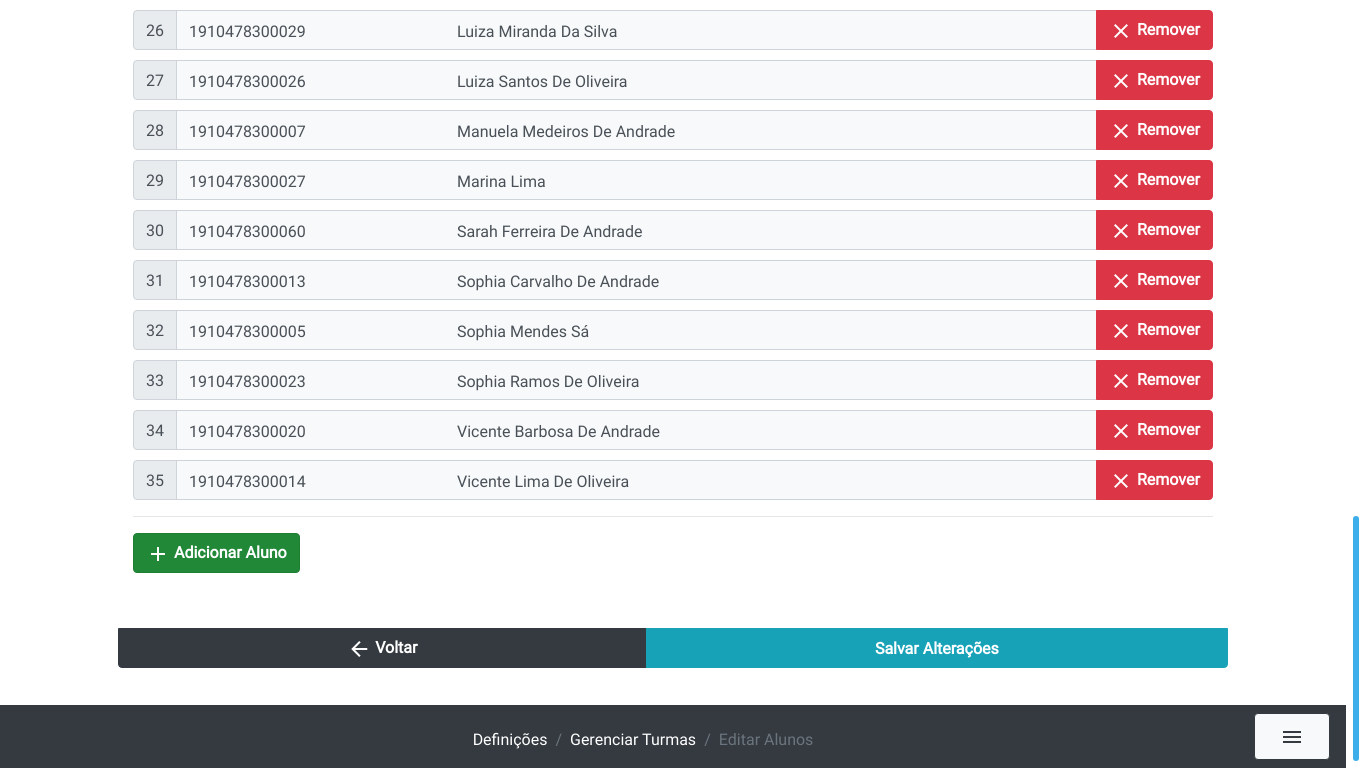
\includegraphics[width=0.8\textwidth]{TCC/imagens/sistema/10b.png}
     \caption{Tela de Edição de Turmas -- Cont.}
     \label{tela-edit-2}
\end{figure}

Para se \textbf{apagar uma turma}, uma mensagem irá informar que, ao apagar a turma ela não poderá ser recuperada posteriormente (figura \ref{tela-delete}).

%% Apagar turma
\begin{figure}[H]
     \centering
     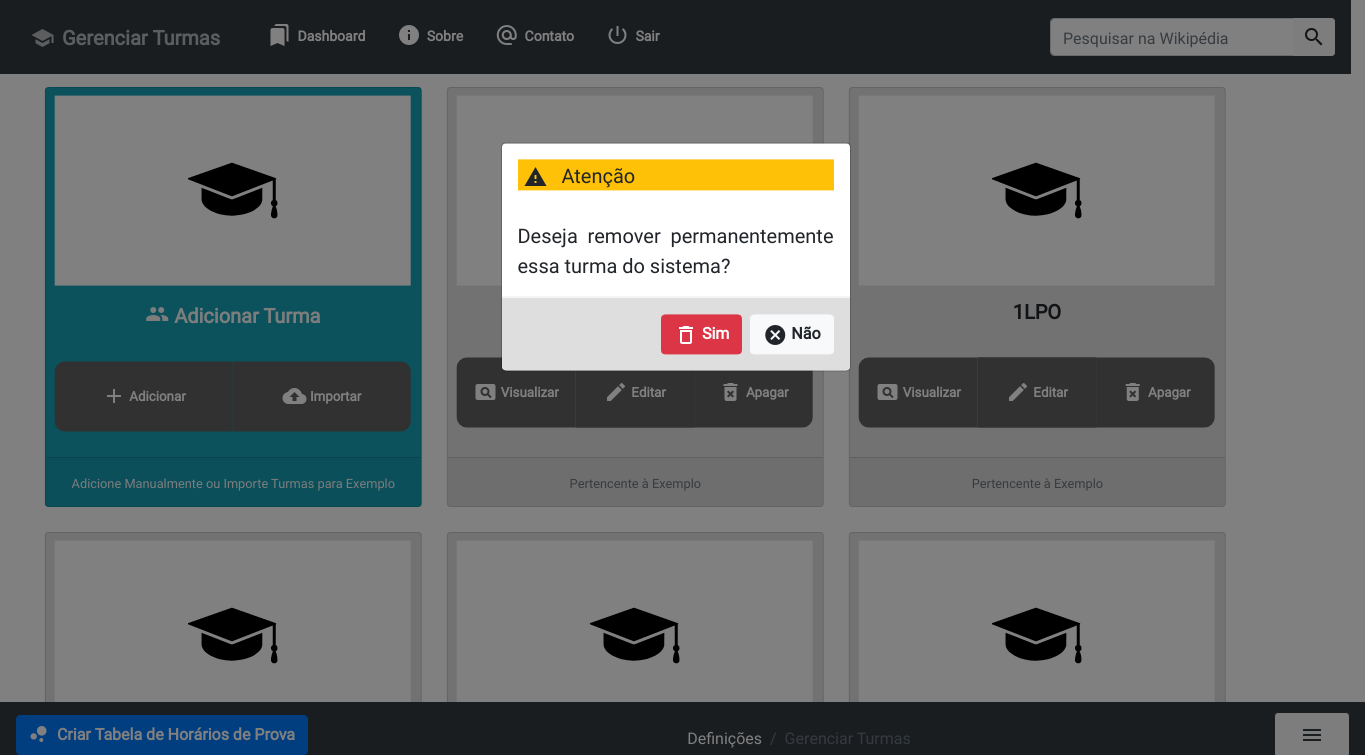
\includegraphics[width=0.8\textwidth]{TCC/imagens/sistema/11.png}
     \caption{Notificação ao Apagar Turma}
     \label{tela-delete}
\end{figure}

Para criar uma nova turma o usuário deverá \textbf{Adicionar Turma} na tela de \textbf{Gerenciamento de Turmas} (conforme na figura \ref{tela-gerenciador}), e para incluir a nova turma deverá informar o nome dessa turma (figura \ref{tela-create}), e opcionalmente deverá informar os alunos que a compõe, informando a matrícula e o nome completo do aluno (figura \ref{tela-create-2}).
%% Criar turma 1
\begin{figure}[H]
     \centering
     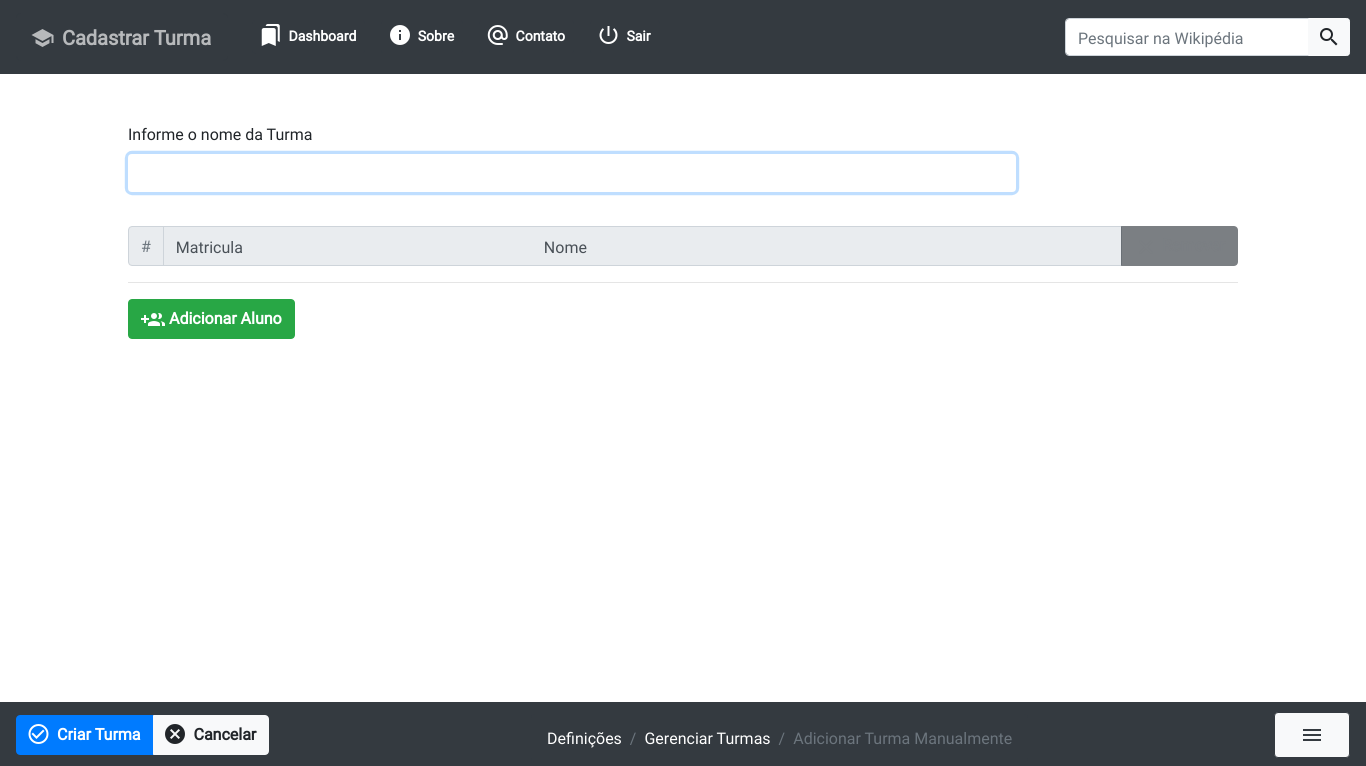
\includegraphics[width=0.8\textwidth]{TCC/imagens/sistema/14.png}
     \caption{Tela de Criação de Nova Turma}
     \label{tela-create}
\end{figure}

%% Criar turma 2
\begin{figure}[H]
     \centering
     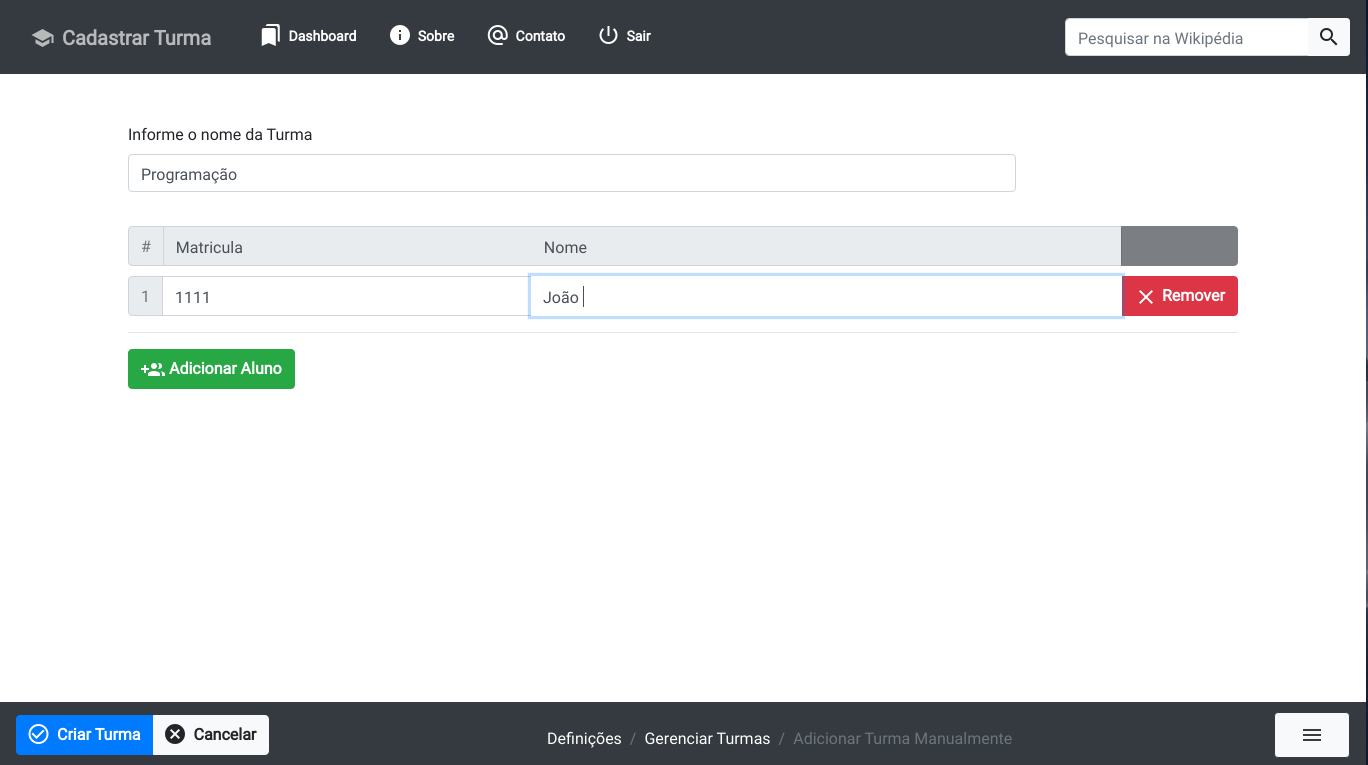
\includegraphics[width=0.8\textwidth]{TCC/imagens/sistema/14a.png}
     \caption{Tela de Criação de Nova Turma -- Cont.}
     \label{tela-create-2}
\end{figure}

Outra opção na página de Gerenciamento de turmas é a \textbf{inclusão de turmas por importação de um arquivo XSLX} (planilha \textit{MS Excel}), que deve estar formatada de acordo com o padrão do sistema e assim só será necessário realizar o \textit{update} do arquivo clicando em enviar e as turmas serão importadas para o espaço de trabalho (figura \ref{tela-import}).

%% Importar turmas de planilha
\begin{figure}[H]
     \centering
     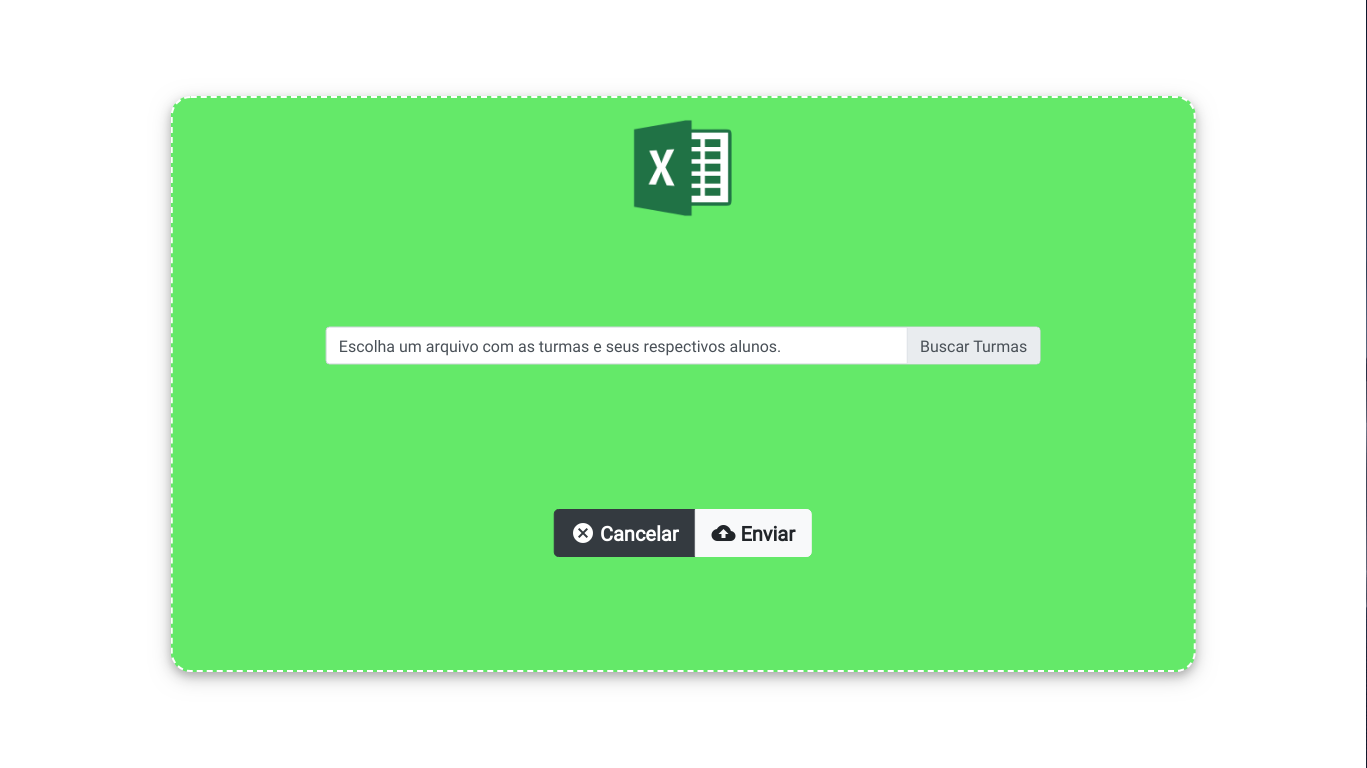
\includegraphics[width=0.8\textwidth]{TCC/imagens/sistema/15.png}
     \caption{Tela de Importação de Turmas por Arquivo}
     \label{tela-import}
\end{figure}

\subsection{Alocar Turmas em Horários de Prova}

A tela onde iremos \textbf{alocar as turmas nos horários de prova} é a principal página do sistema, pois é aqui que criaremos as tabelas de horários de prova (figura \ref{tela-aloc-2h}). Devemos informar nessa página a quantidade de horários que dispomos para realizar as provas (na figura \ref{tela-aloc-3h} foi definido que existem três horários disponíveis para realizar a prova).
%% Alocar 1
\begin{figure}[H]
     \centering
     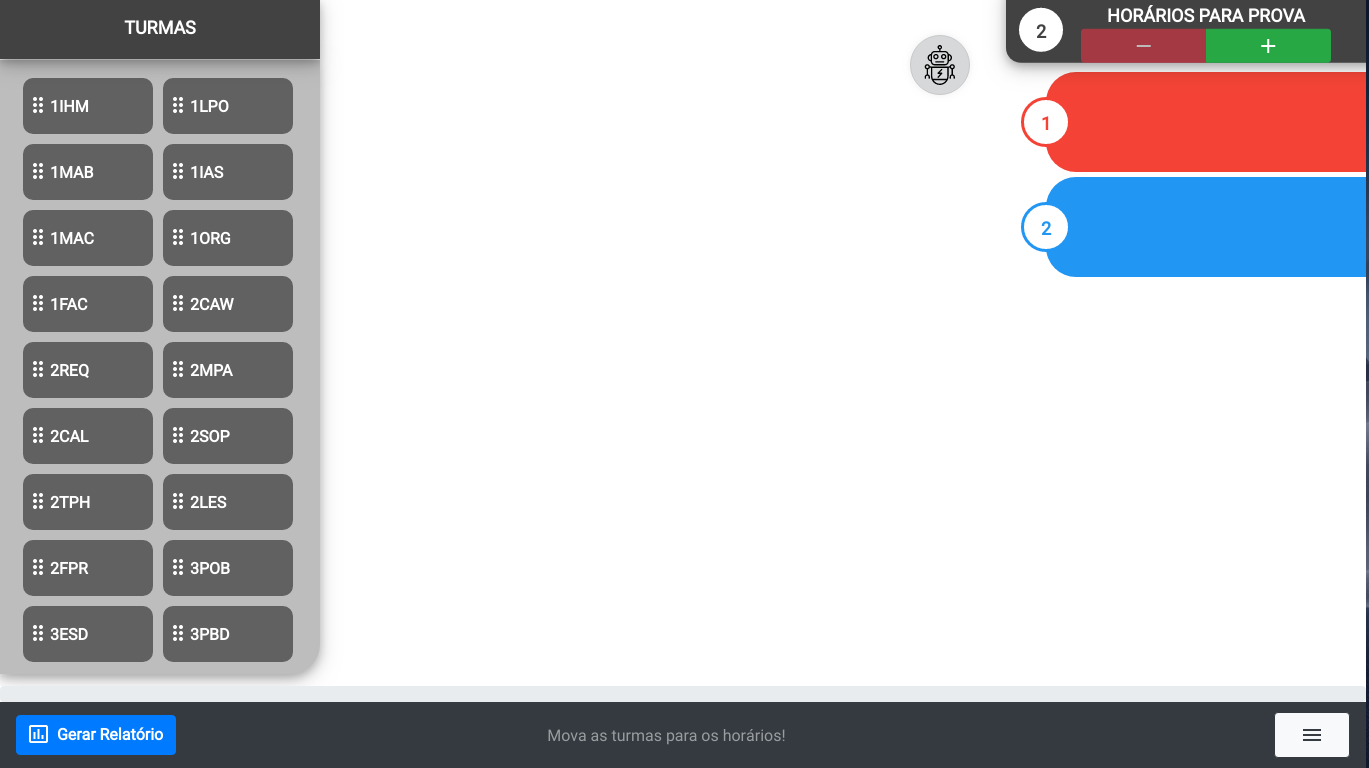
\includegraphics[width=0.8\textwidth]{TCC/imagens/sistema/12a.png}
     \caption{Tela de Alocar Turmas em 2 Horários}
     \label{tela-aloc-2h}
\end{figure}

%% Alocar 2
\begin{figure}[H]
     \centering
     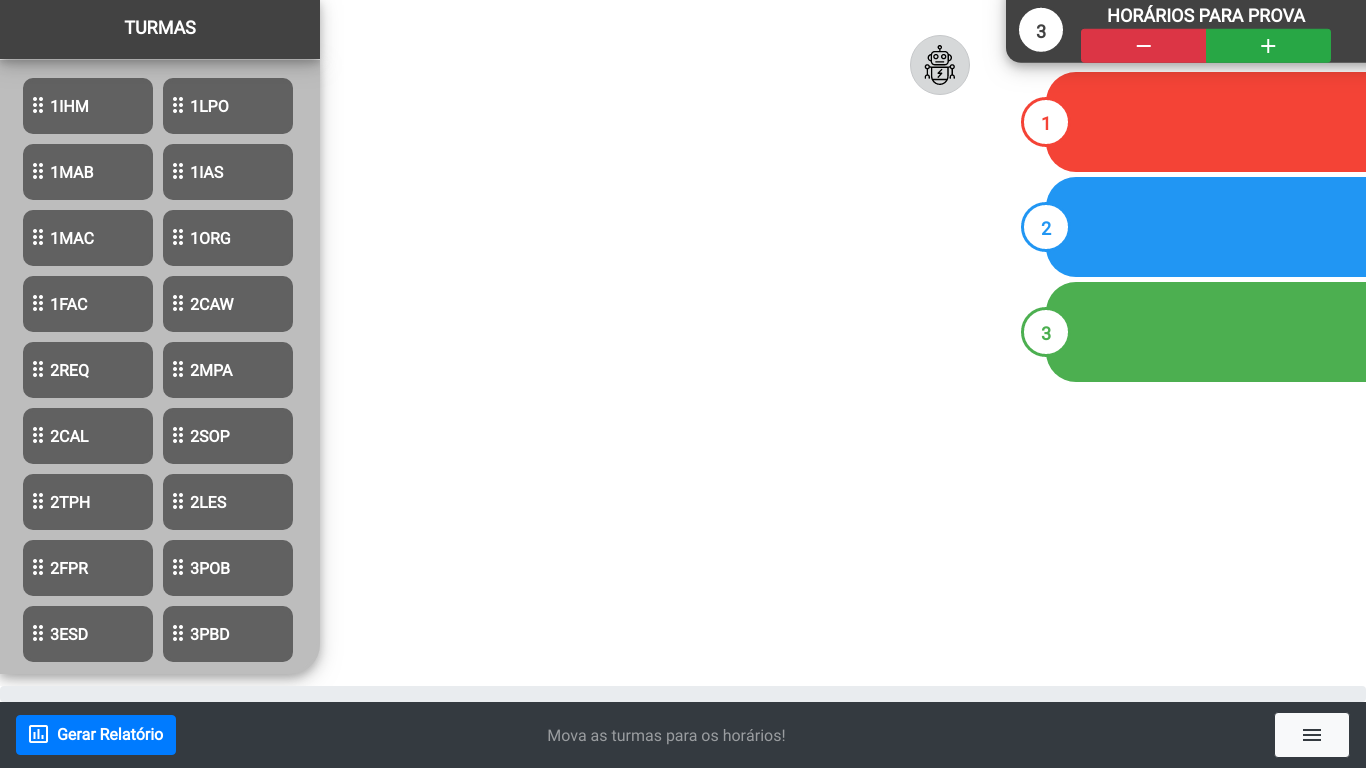
\includegraphics[width=0.8\textwidth]{TCC/imagens/sistema/12b.png}
     \caption{Tela de Alocar Turmas em 3 Horários}
     \label{tela-aloc-3h}
\end{figure}

Na barra situada na parte de baixo na página temos o menu secundário (figura \ref{tela-aloc-menu}), que apresenta as opções referentes ao espaço de trabalho e as turmas, assim como opções já apresentadas.
%% Alocar 1
\begin{figure}[H]
     \centering
     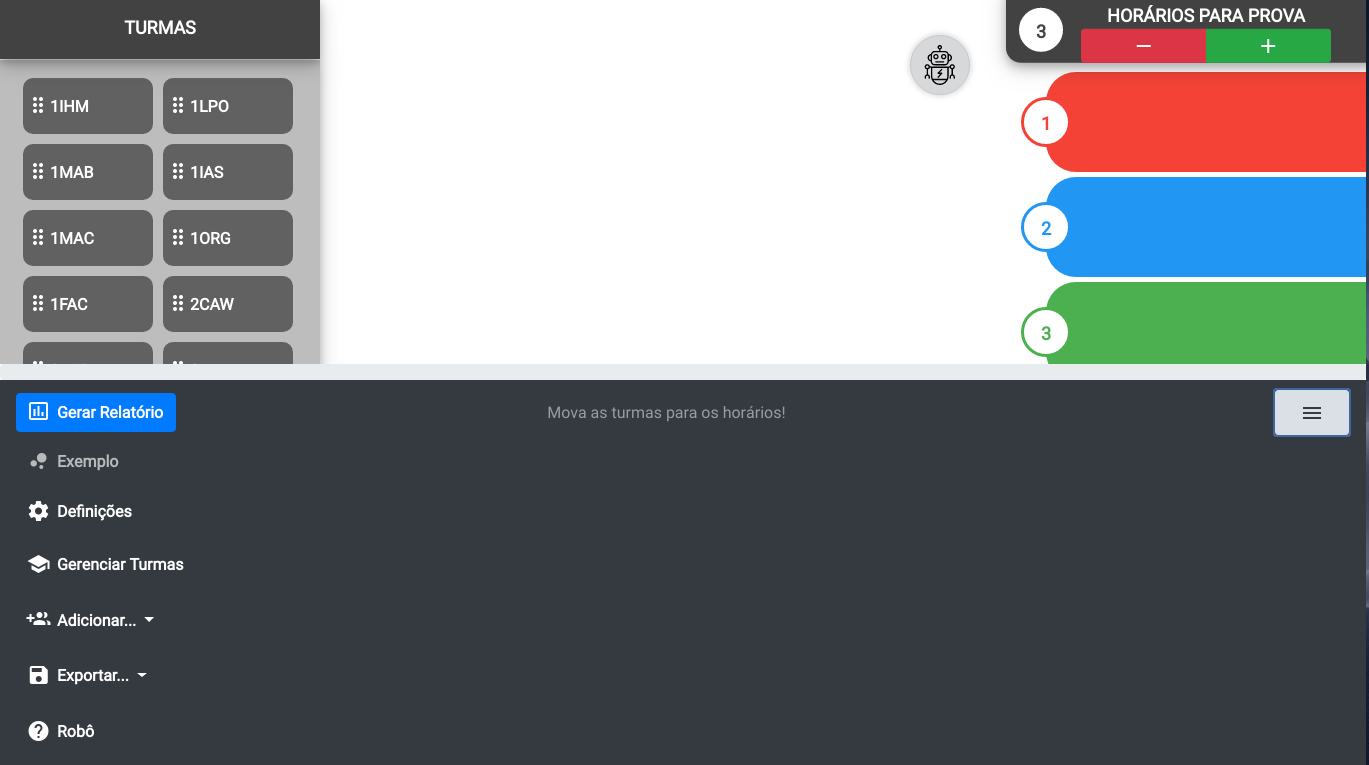
\includegraphics[width=0.8\textwidth]{TCC/imagens/sistema/12b-2.png}
     \caption{Tela de Alocar Turmas em 3 Horários -- Menu}
     \label{tela-aloc-menu}
\end{figure}


%% ===========================================================
%% ===========   EXEMPLO DE ALOCAÇÃO DE TURMAS ===============

    \begin{table}[h]
        \centering
        \caption{Exemplos de alocações e seus resultados}
        \vspace{0.5cm}
        \renewcommand\arraystretch{1.5}
        \begin{tabular}{c|c|c|c|c}
         
            \textbf{Figura} & \textbf{Moveu as Turmas} & \textbf{Para os Horários}  & \textbf{Conflitos} & \textbf{Taxa de Conflitos}\\ % Note a separação de col. e a quebra de linhas
            \hline                               % para uma linha horizontal
            \ref{tela-aloc-ex1} &   1HM  &   1  &    0   & 0\% \\
            \ref{tela-aloc-ex2} &   1IAS  &   2  &    0   & 0\% \\
            \ref{tela-aloc-ex3} &   1MAB  &   3  &    0   & 0\% \\
            \ref{tela-aloc-ex4} &  1LPO e 1IAS   &   2 e 1  &    8   & 15\% \\ 
            \ref{tela-aloc-ex5} &  1MAC e 1ORG   &  2 e 3   &    26   & 19\% \\ 
            \ref{tela-aloc-ex6} &   TODAS  &   1  &    140   & 100\% \\ 
            \ref{tela-aloc-ex7} &   1LPO, 1MAB, 1IAS  &   2  &    57   & 41\%
            % não é preciso quebrar a última linha
            \\
            \hline
        \end{tabular}
        \label{tabela-exemplo}
    \end{table}

Para se alocar uma turma em um horário basta clicar na turma, manter pressionado e arrastar até o \textbf{\textit{slot}} de horário desejado. Na tabela \ref{tabela-exemplo} temos descrita uma sequência de movimentações para exemplificar o funcionamento dessa tela. 

Os conflitos são correspondentes ao número de provas de segunda chamada, necessárias para a realização daquela tabela de horários de prova. 

A taxa de conflitos é obtida através do maior número de conflito possível para as turmas selecionadas, divido pela quantidade de conflitos da solução atual multiplicado por 100.






%% ===========================================================

%% Alocar 2
\begin{figure}[H]
     \centering
     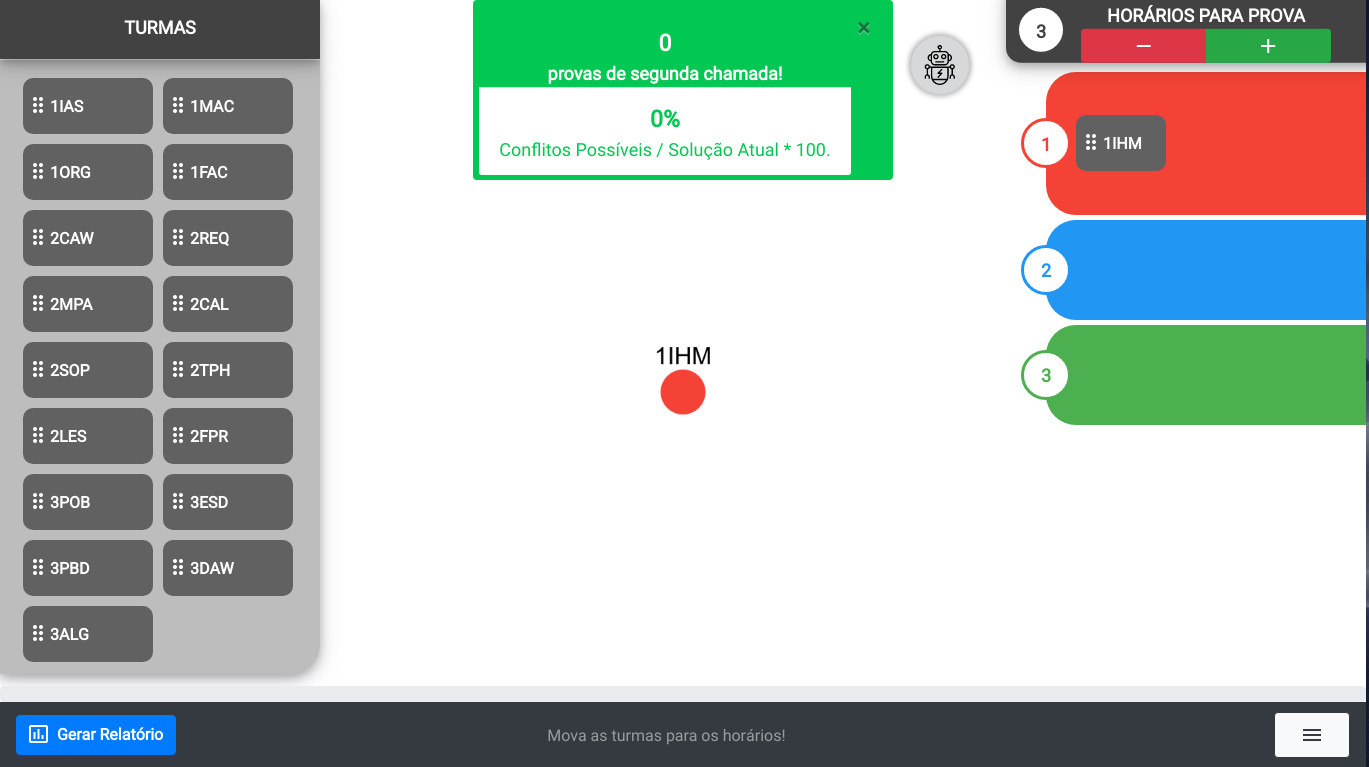
\includegraphics[width=0.8\textwidth]{TCC/imagens/sistema/12c.png}
     \caption{Tela de Alocar Turmas -- Exemplo 1}
     \label{tela-aloc-ex1}
\end{figure}

%% Alocar 1
\begin{figure}[H]
     \centering
     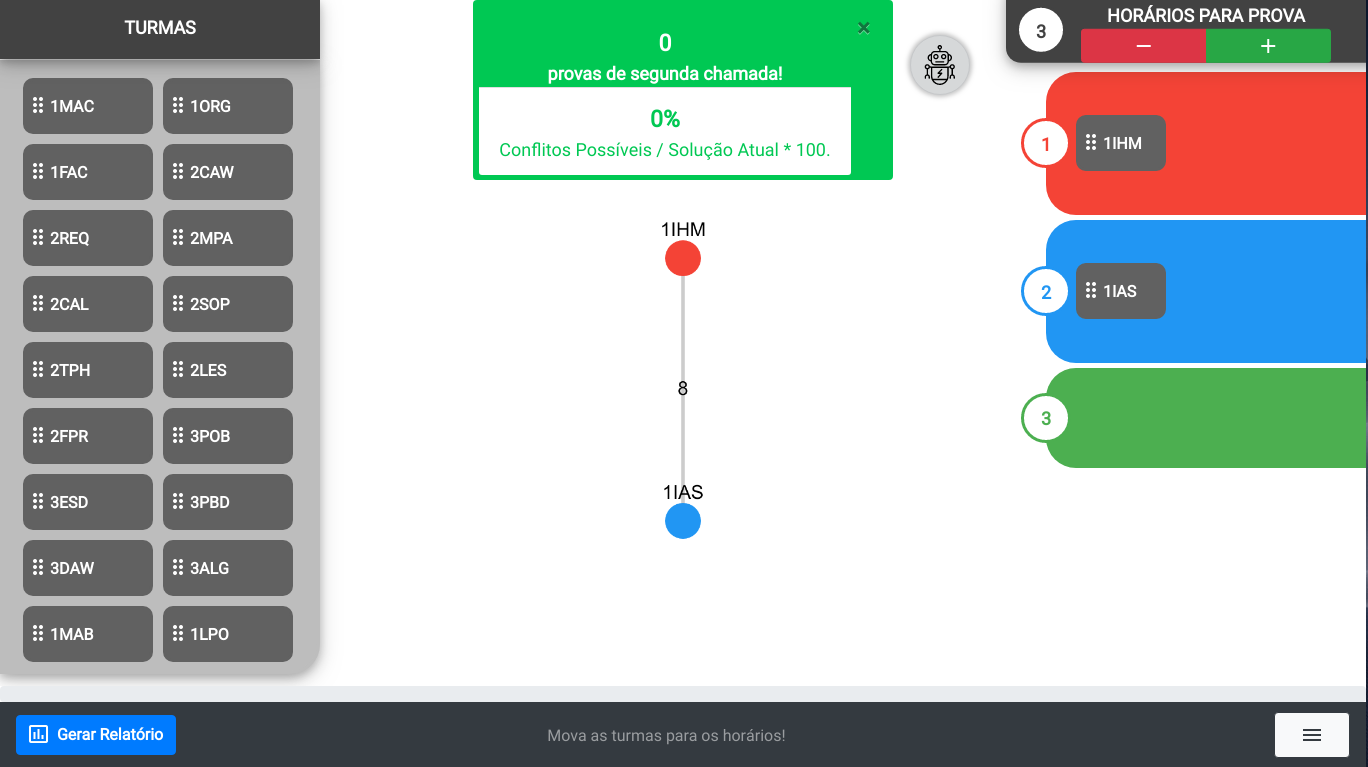
\includegraphics[width=0.8\textwidth]{TCC/imagens/sistema/12d.png}
     \caption{Tela de Alocar Turmas -- Exemplo 2}
     \label{tela-aloc-ex2}
\end{figure}

%% Alocar 2
\begin{figure}[H]
     \centering
     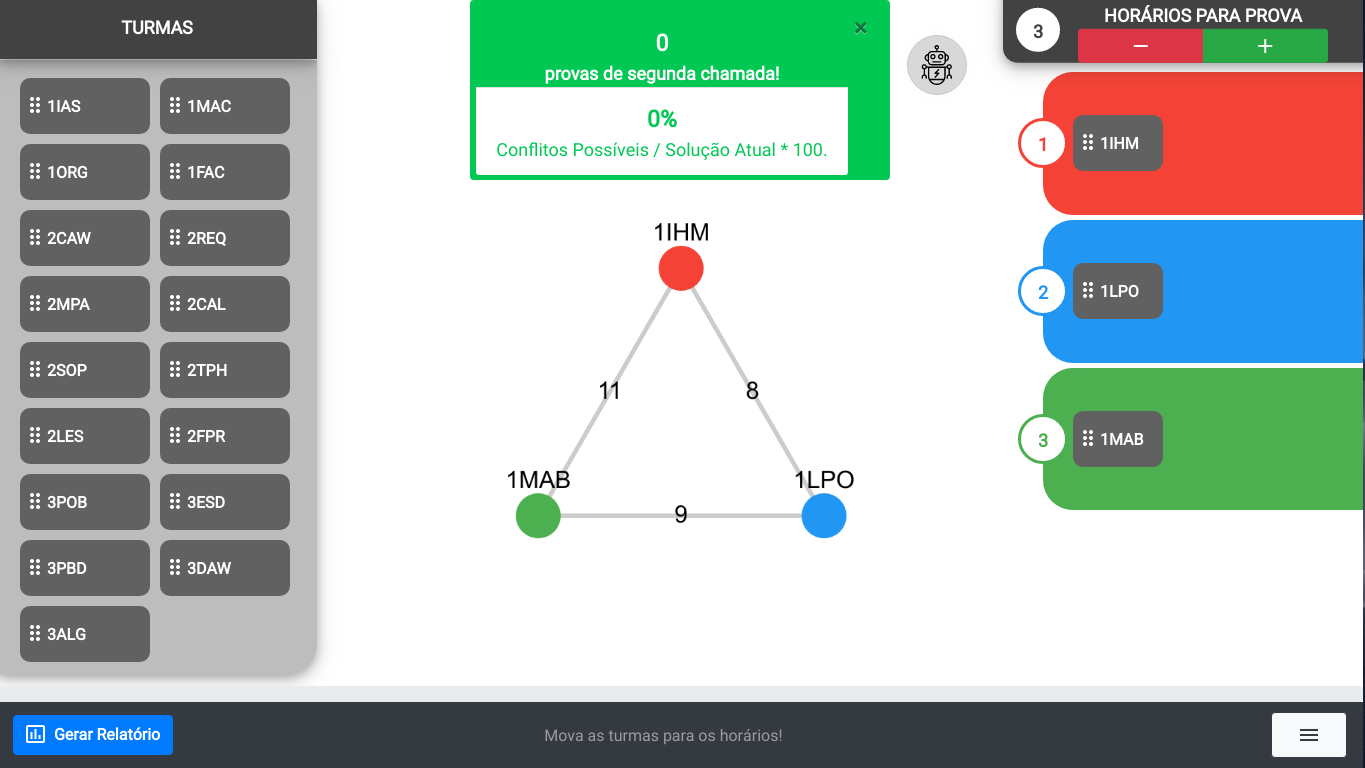
\includegraphics[width=0.8\textwidth]{TCC/imagens/sistema/12e.png}
     \caption{Tela de Alocar Turmas -- Exemplo 3}
     \label{tela-aloc-ex3}
\end{figure}

%% Alocar 1
\begin{figure}[H]
     \centering
     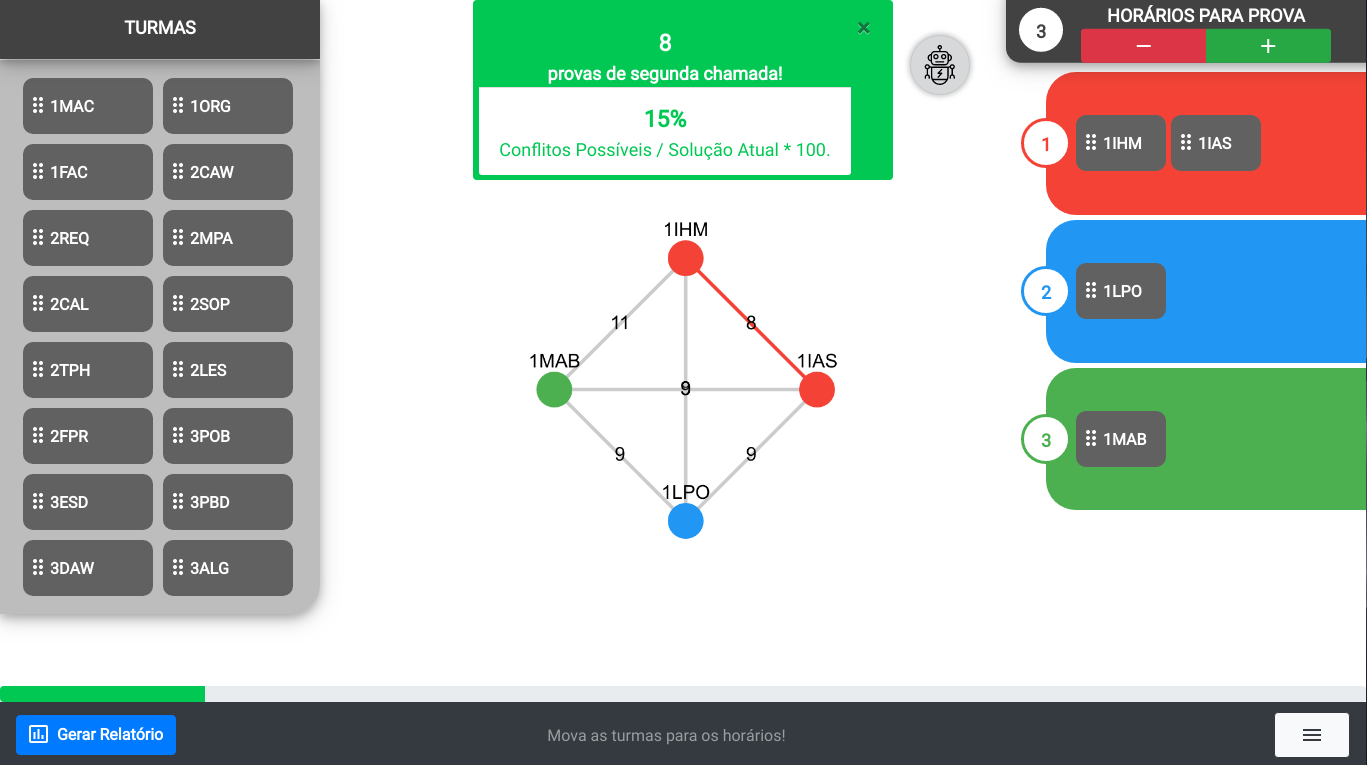
\includegraphics[width=0.8\textwidth]{TCC/imagens/sistema/12f.png}
     \caption{Tela de Alocar Turmas -- Exemplo 4}
     \label{tela-aloc-ex4}
\end{figure}

%% Alocar 2
\begin{figure}[H]
     \centering
     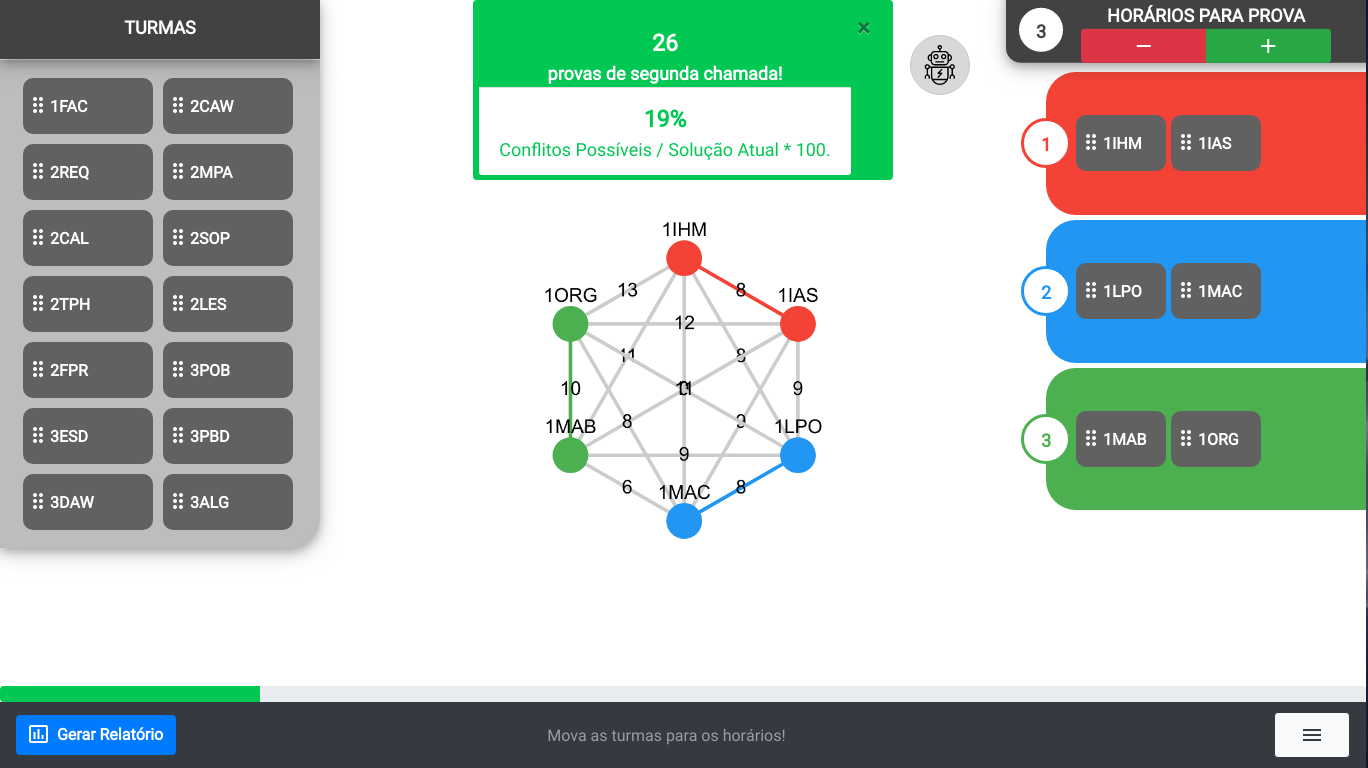
\includegraphics[width=0.8\textwidth]{TCC/imagens/sistema/12g.png}
     \caption{Tela de Alocar Turmas -- Exemplo 5}
     \label{tela-aloc-ex5}
\end{figure}



%% Alocar 2
\begin{figure}[H]
     \centering
     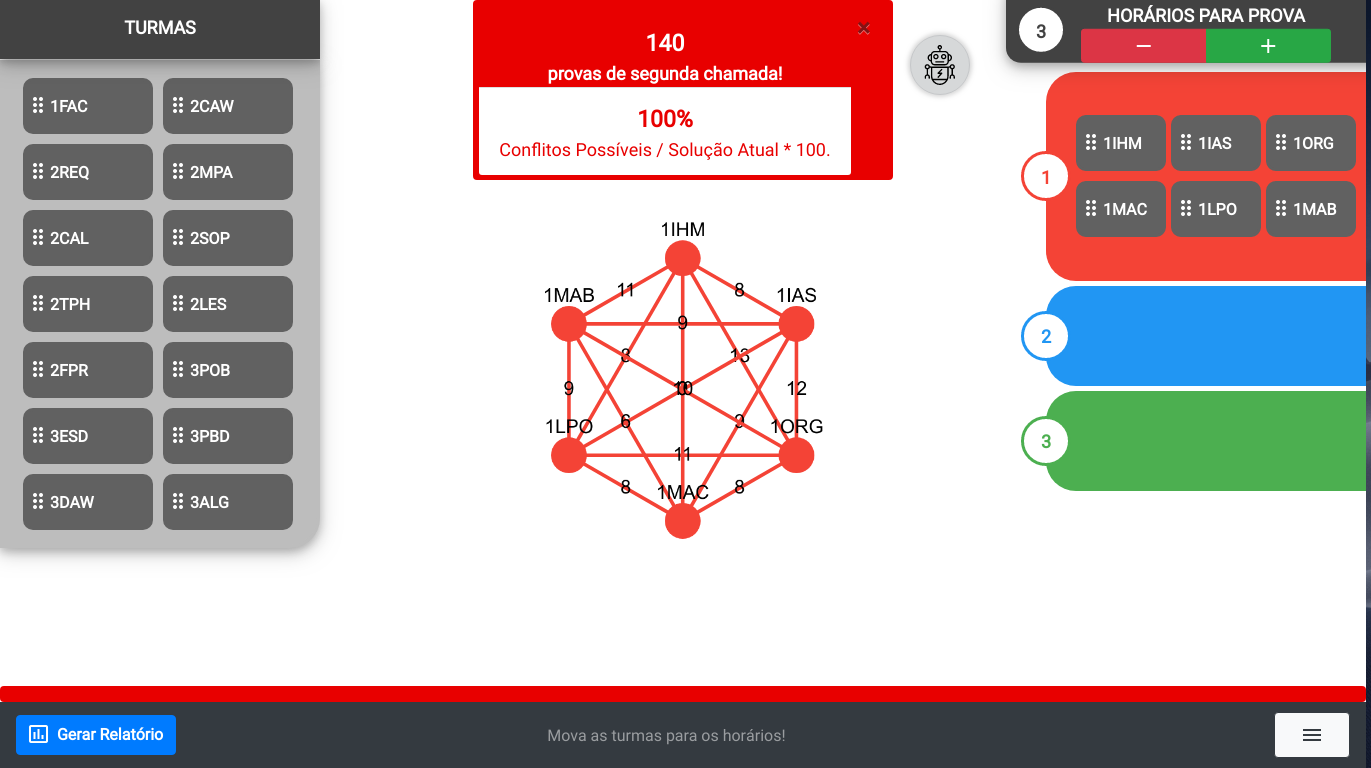
\includegraphics[width=0.8\textwidth]{TCC/imagens/sistema/12h.png}
     \caption{Tela de Alocar Turmas -- Exemplo 6}
     \label{tela-aloc-ex6}
\end{figure}

%% Alocar 2
\begin{figure}[H]
     \centering
     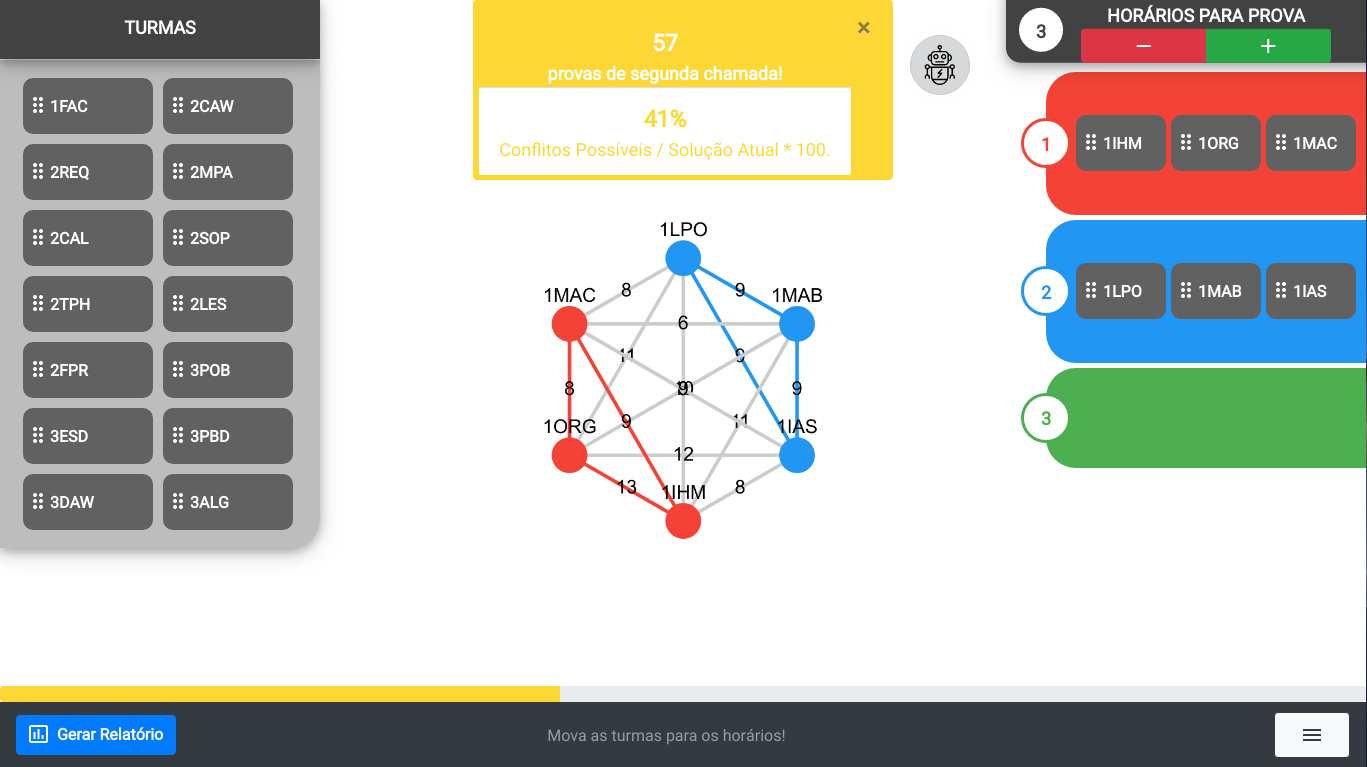
\includegraphics[width=0.8\textwidth]{TCC/imagens/sistema/12i.png}
     \caption{Tela de Alocar Turmas -- Exemplo 7}
     \label{tela-aloc-ex7}
\end{figure}



 





\subsection{Gerar Relatório da Alocação}
%% ===========================================================
%% ===========   EXEMPLO DE GERAÇÃO DE RESULTADO =============


Agora vamos usar a tabela de horários de prova mostrada na figura \ref{tela-grade1} como a grade de horários que desejamos utilizar, dessa forma podemos clicar no botão \textbf{Gerar Relatório} para concluir a alocação das turmas e visualizar o resultado de forma detalhada como nas figuras \ref{tela-grade2} e \ref{tela-grade3}.

Na figura \ref{tela-grade4} percebemos que em caso de clicarmos na linha da imagem (aresta do Grafo) será exibido os alunos que pertencem as duas turmas que a linha conecta. Já na figura \ref{tela-grade5} vemos que ao clicar na turma (no vértice do Grafo) temos a lista com todos os alunos pertencentes aquela turma.

%% ===========================================================
%% Alocando Turmas 1
\begin{figure}[H]
     \centering
     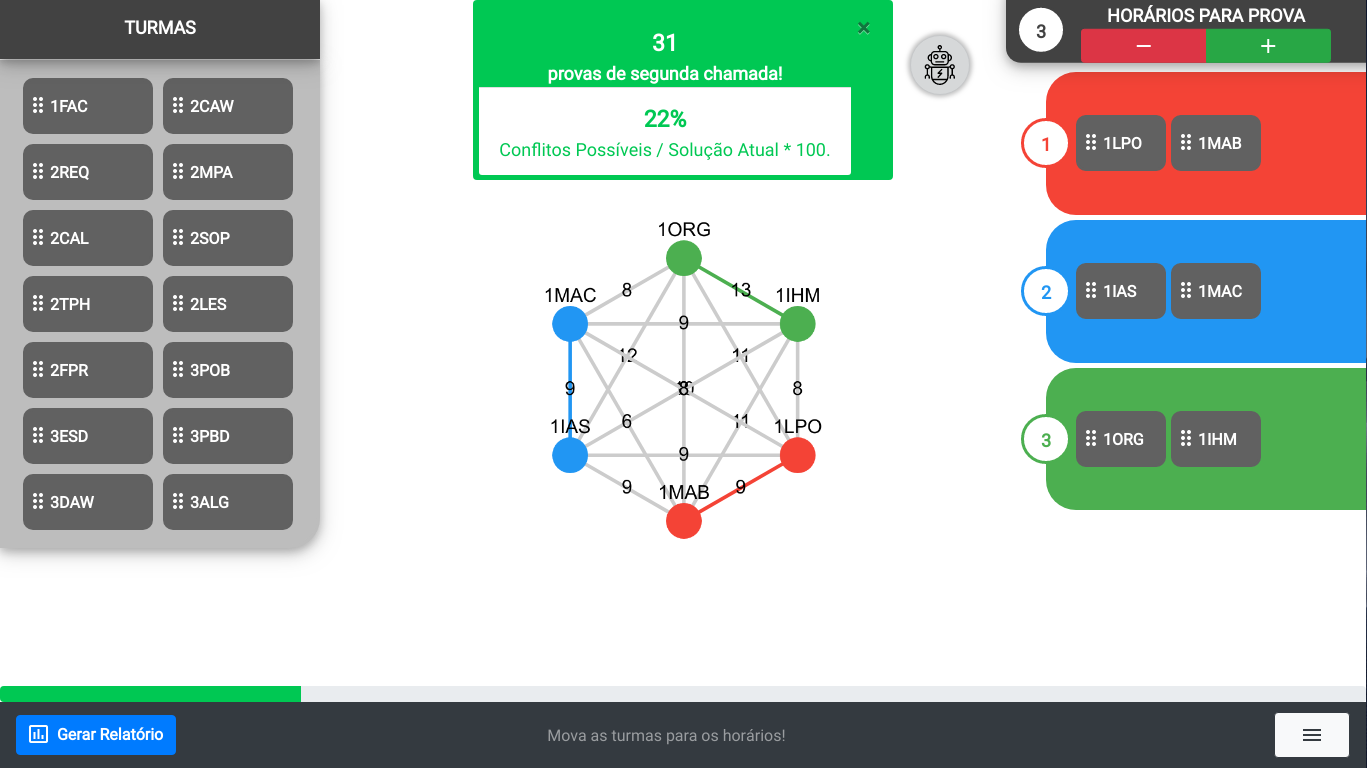
\includegraphics[width=0.8\textwidth]{TCC/imagens/sistema/13a.png}
     \caption{Gerando uma Grade de Prova -- pt. 1}
     \label{tela-grade1}
\end{figure}

%% Alocando Turmas 2
\begin{figure}[H]
     \centering
     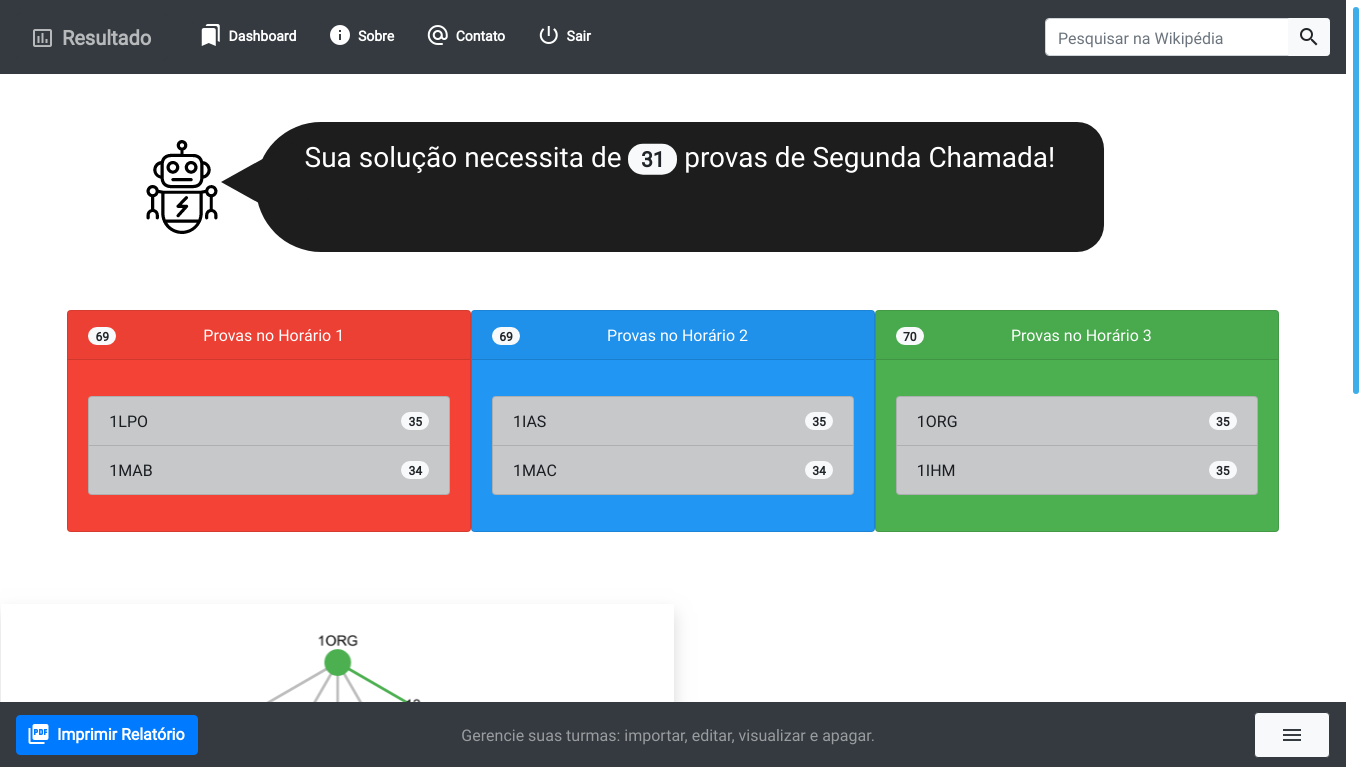
\includegraphics[width=0.8\textwidth]{TCC/imagens/sistema/13b-1.png}
     \caption{Gerando uma Grade de Prova -- pt. 2}
     \label{tela-grade2}
\end{figure}



%% Alocando Turmas 3
\begin{figure}[H]
     \centering
     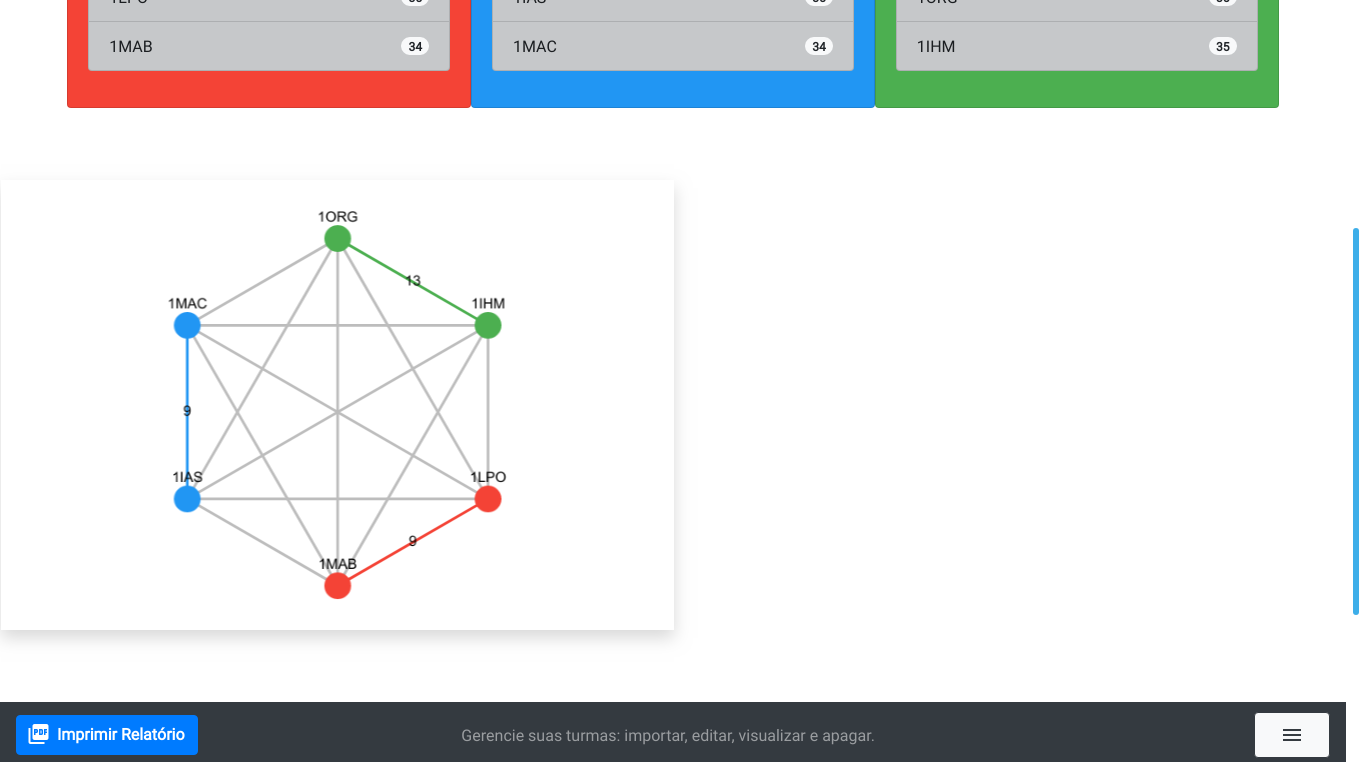
\includegraphics[width=0.8\textwidth]{TCC/imagens/sistema/13b-2.png}
     \caption{Gerando uma Grade de Prova -- pt. 3}
     \label{tela-grade3}
\end{figure}

%% Alocando Turmas 4
\begin{figure}[H]
     \centering
     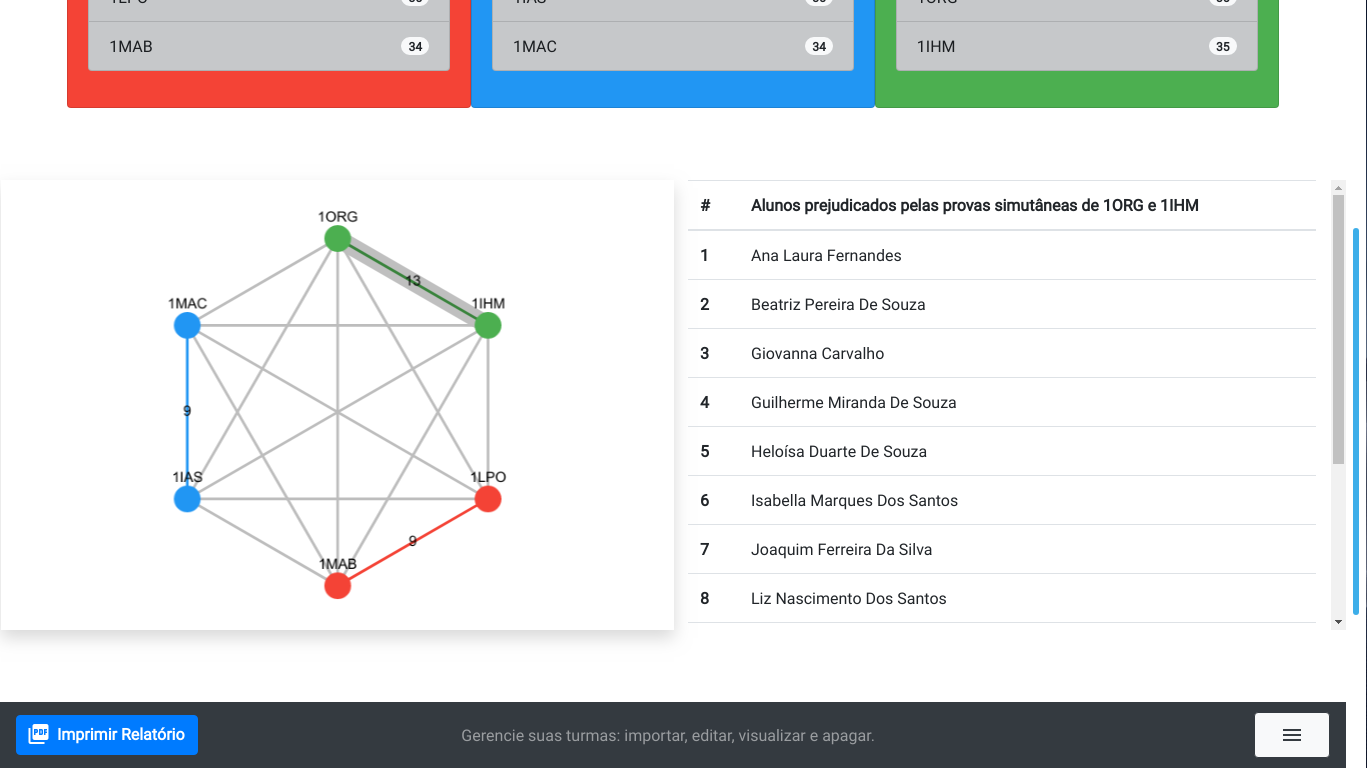
\includegraphics[width=0.8\textwidth]{TCC/imagens/sistema/13b-3.png}
     \caption{Gerando uma Grade de Prova -- pt. 4}
     \label{tela-grade4}
\end{figure}

%% Alocando Turmas 5
\begin{figure}[H]
     \centering
     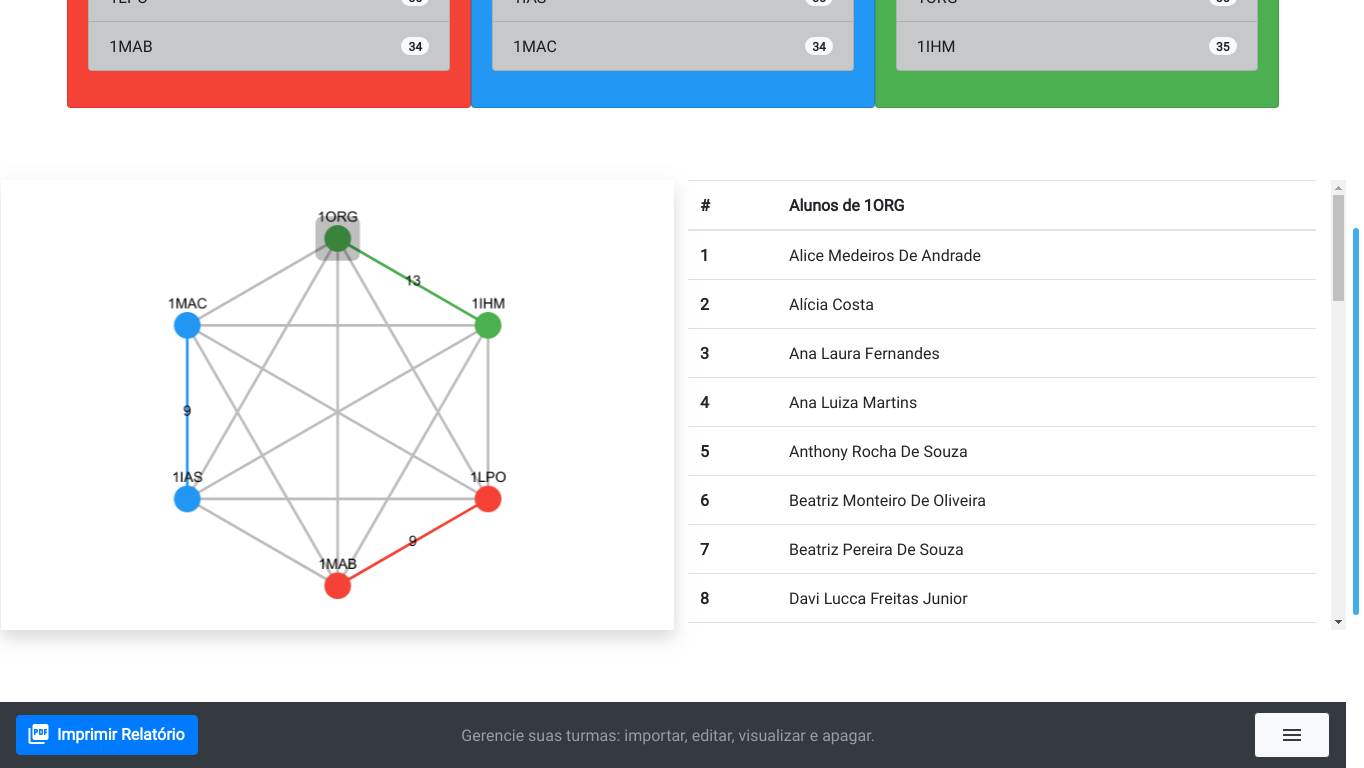
\includegraphics[width=0.8\textwidth]{TCC/imagens/sistema/13b-4.png}
     \caption{Gerando uma Grade de Prova -- pt. 5}
     \label{tela-grade5}
\end{figure}

Ao final da página de relatório temos uma opção descrita como "Deseja tentar encontrar um resultado melhor usando nosso robô?"\ (figura \ref{tela-grade6}), essa opção irá utilizar o algoritmo criado para o sistema para buscar a melhor distribuição de turmas nos horários, isto é a alocação que vai gerar o menor número de provas de segunda chamada por conflitos de horário. 


%% Alocando Turmas 6
\begin{figure}[H]
     \centering
     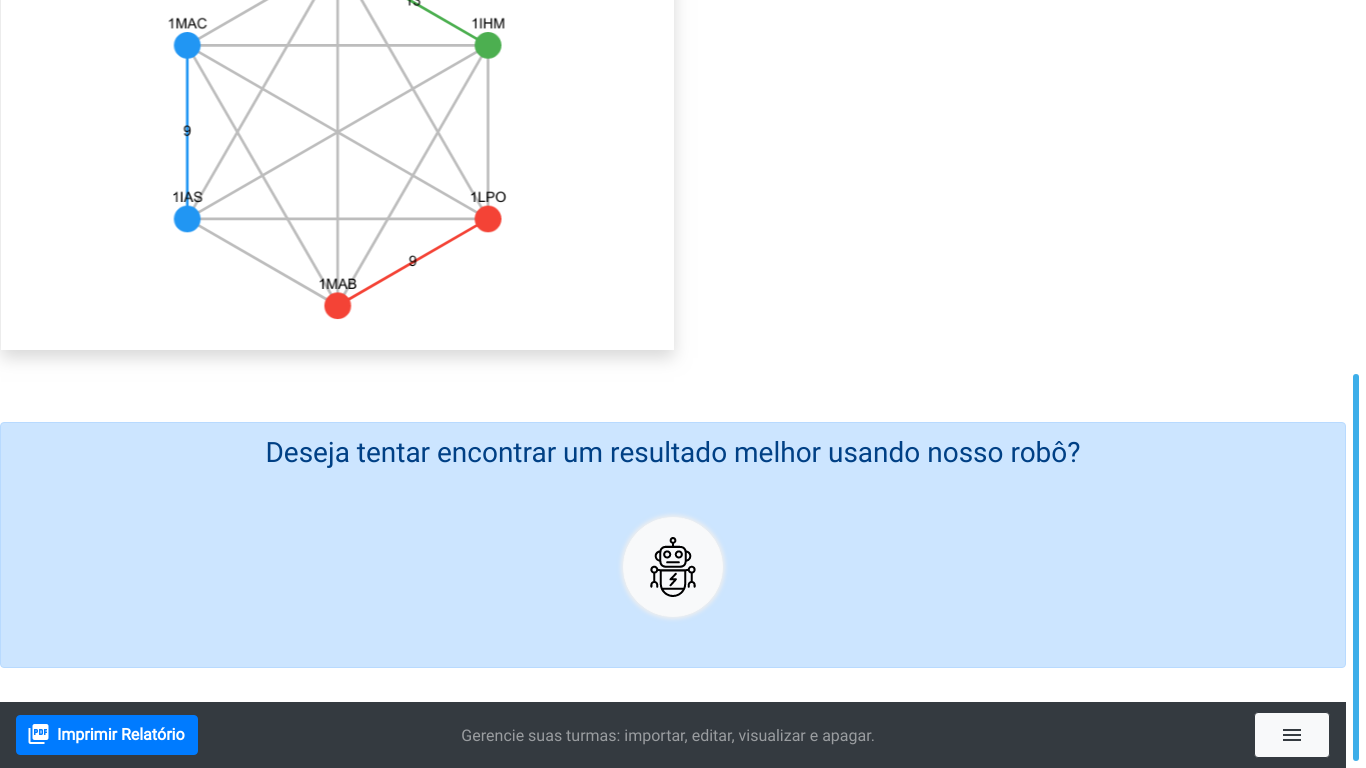
\includegraphics[width=0.8\textwidth]{TCC/imagens/sistema/13b-5.png}
     \caption{Gerando uma Grade de Prova -- pt. 6}
     \label{tela-grade6}
\end{figure}

Caso o usuário opte por essa opção ele será redirecionado para uma nova página de \textbf{relatório} (figura \ref{tela-grade7}). 

Vale dizer que caso o usuário clicasse no \textbf{botão do "Robô"}\ na página de\textbf{ criação de tabela de horário} (figuras \ref{tela-aloc-2h} e \ref{tela-aloc-3h} ele seria direcionado para esse mesmo relatório.

Vemos na figura \ref{tela-grade7} que além de apresentar a quantidade de provas necessárias para realização das provas, esse relatório também irá apresentar a quantidade de provas necessárias na solução manual, que foi gerada anteriormente, e o quanto o "Robô"\ conseguiu melhorar o resultado manual. 

Além das diferenças já citadas, a página vai apresentar as mesmas informações quanto aos horários em que as turmas foram alocadas, e uma figura interativa (de um Grafo) que representa a relação entre as turmas, contanto não haverá mais a opção de tentar uma solução melhor com o "Robô"\ já que essa se trata da melhor solução possível (figura \ref{tela-grade8}).


%% Alocando Turmas 5
\begin{figure}[H]
     \centering
     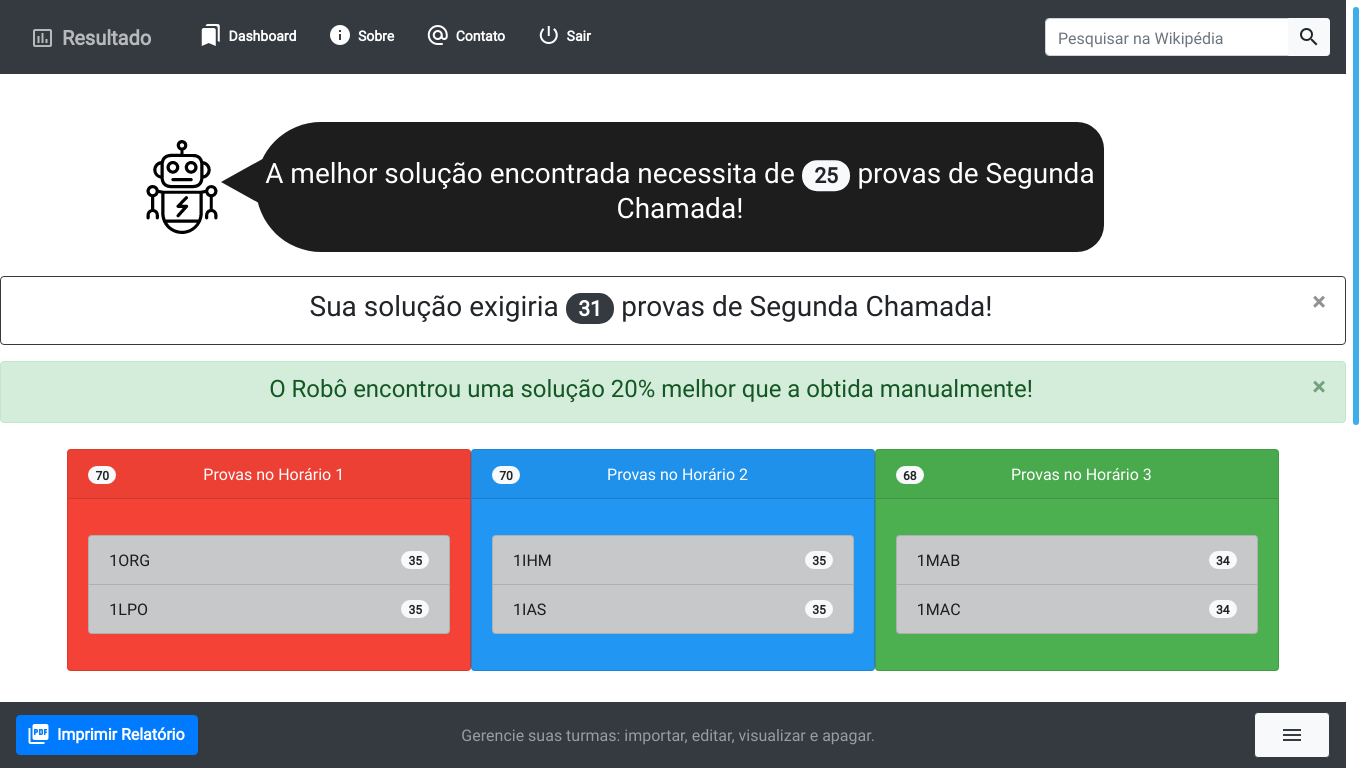
\includegraphics[width=0.8\textwidth]{TCC/imagens/sistema/13c-1.png}
     \caption{Gerando uma Grade de Prova -- pt. 7}
     \label{tela-grade7}
\end{figure}

%% Alocando Turmas 5
\begin{figure}[H]
     \centering
     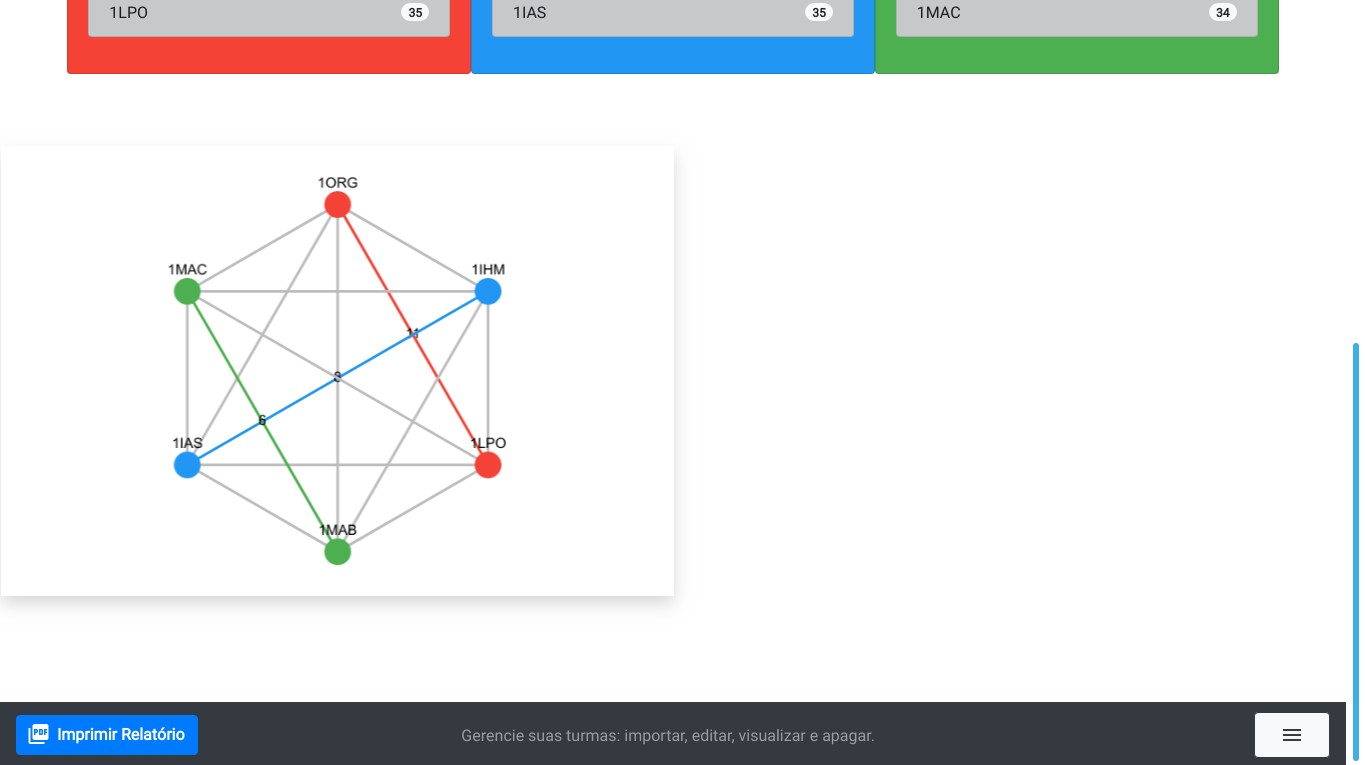
\includegraphics[width=0.8\textwidth]{TCC/imagens/sistema/13c-2.png}
     \caption{Gerando uma Grade de Prova -- pt. 8}
     \label{tela-grade8}
\end{figure}



\subsection{Imprimir Relatório}

Na base da tela de relatório temos o menu secundário com algumas opções semelhantes as que já foram apresentadas (figura \ref{tela-grade9}), e além dessas existe a opção de \textbf{Imprimir Relatório}, a qual possibilita gerar um arquivo para impressão ou para \textit{download} (figura \ref{tela-relatorio}).

%% Alocando Turmas 5
\begin{figure}[H]
     \centering
     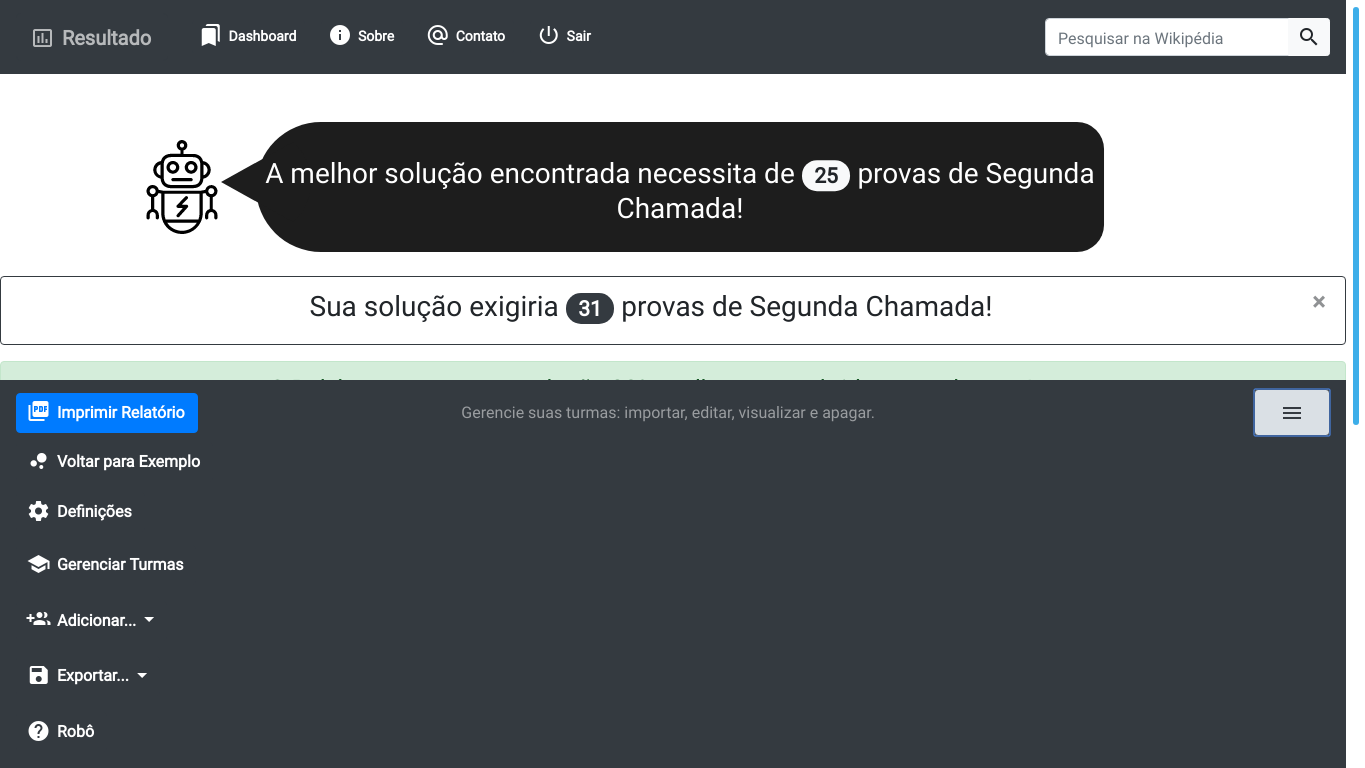
\includegraphics[width=0.8\textwidth]{TCC/imagens/sistema/13c-3.png}
     \caption{Gerando uma Grade de Prova -- pt. 9}
     \label{tela-grade9}
\end{figure}
%% Tela Relatório em PDF
\begin{figure}[H]
     \centering
     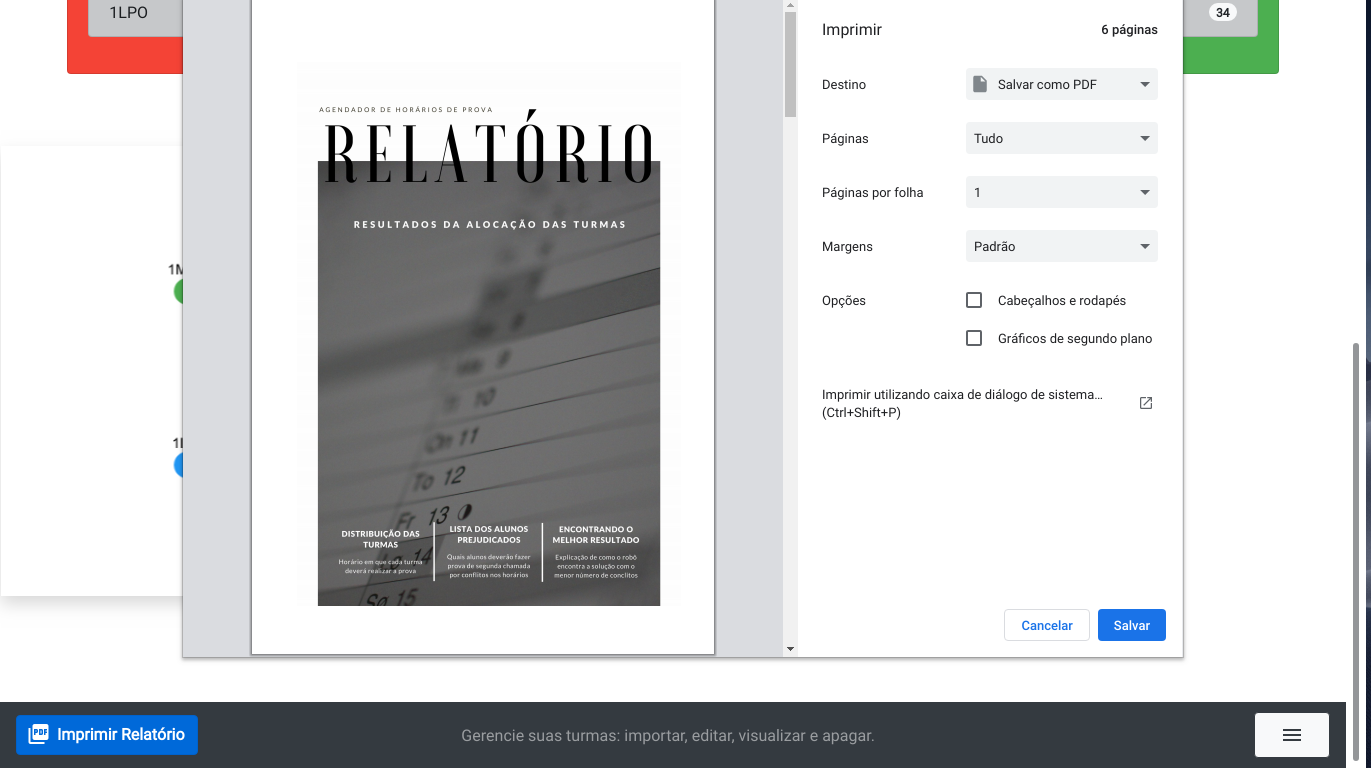
\includegraphics[width=0.8\textwidth]{TCC/imagens/sistema/13d-1.png}
     \caption{Gerando Relatório}
     \label{tela-relatorio}
\end{figure}


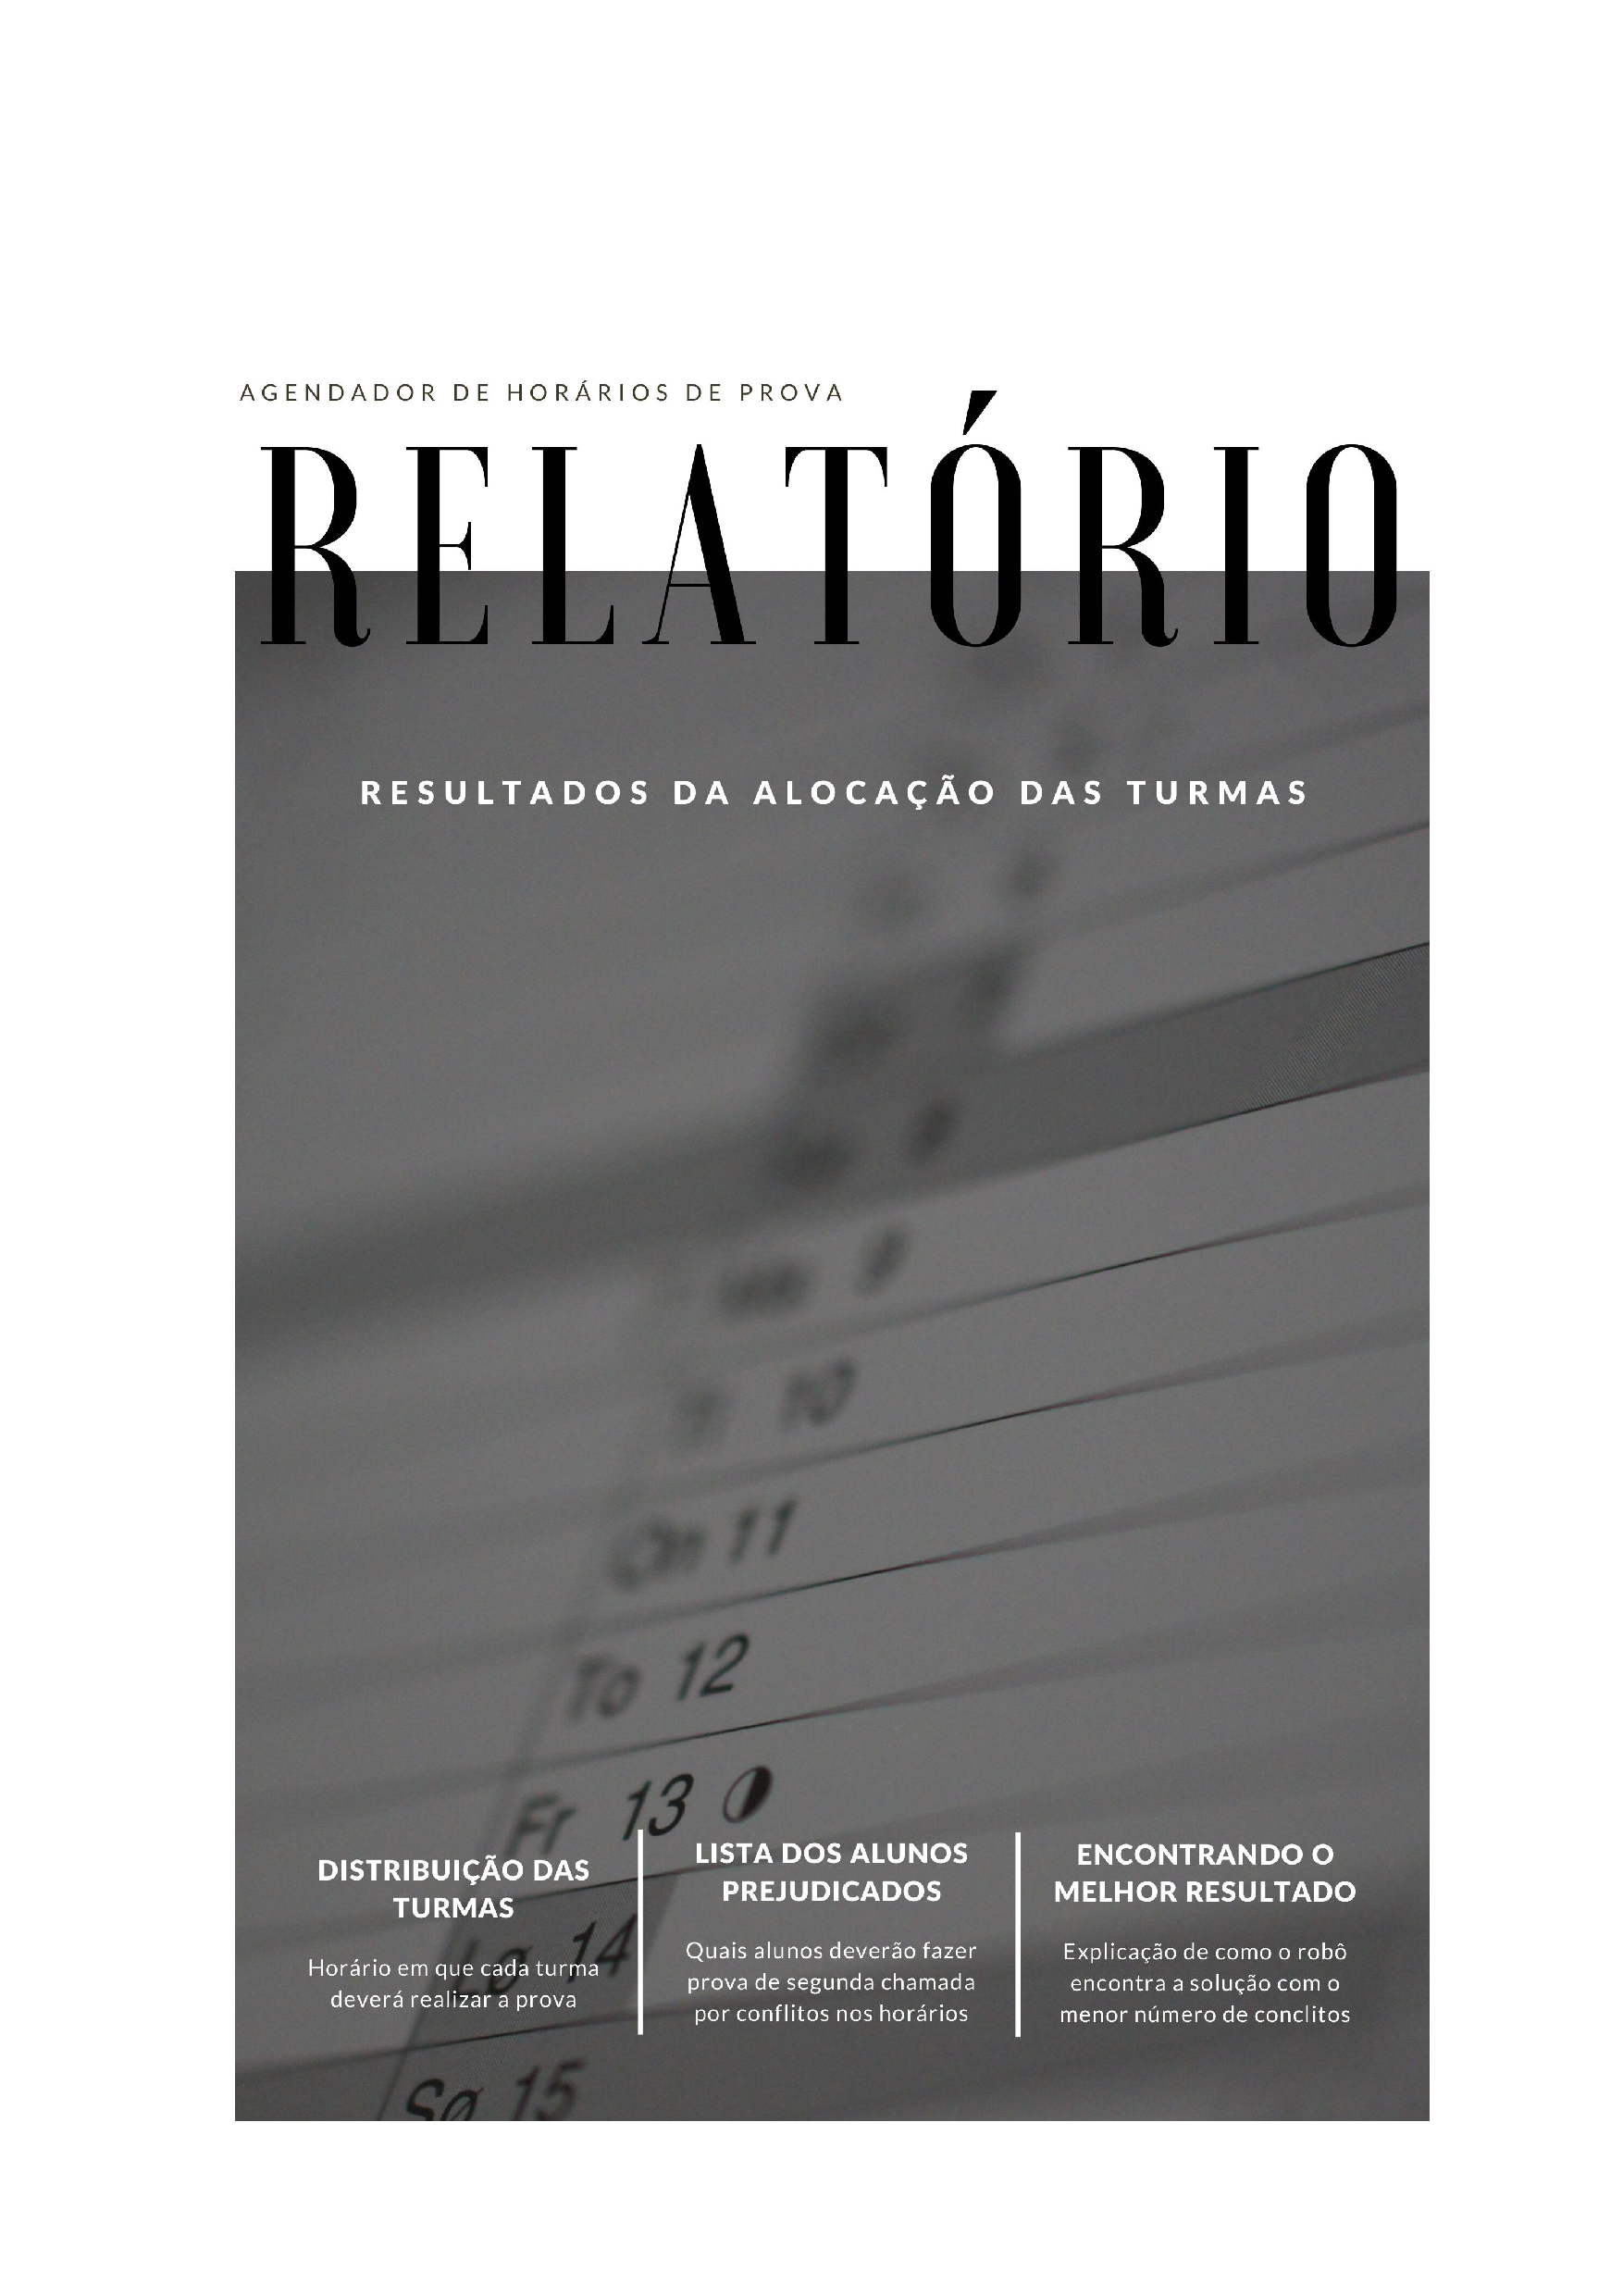
\includepdf[pages=1,pagecommand=\chapter{Relatório}\label{cap:resultado}]{arquivos/anexo-b.pdf}

\end{anexosenv}

\includepdf[pages=2-]{arquivos/anexo-b.pdf}